\documentclass[11pt,fleqn]{book} % Default font size and left-justified equations

%%%%%%%%%%%%%%%%%%%%%%%%%%%%%%%%%%%%%%%%%%%%
%               Structure
%%%%%%%%%%%%%%%%%%%%%%%%%%%%%%%%%%%%%%%%%%%%
%%%%%%%%%%%%%%%%%%%%%%%%%%%%%%%%%%%%%%%%%
% The Legrand Orange Book
% Structural Definitions File
% Version 2.0 (9/2/15)
%
% Original author:
% Mathias Legrand (legrand.mathias@gmail.com) with modifications by:
% Vel (vel@latextemplates.com)
% 
% This file has been downloaded from:
% http://www.LaTeXTemplates.com
%
% License:
% CC BY-NC-SA 3.0 (http://creativecommons.org/licenses/by-nc-sa/3.0/)
%
%%%%%%%%%%%%%%%%%%%%%%%%%%%%%%%%%%%%%%%%%

%----------------------------------------------------------------------------------------
%	VARIOUS REQUIRED PACKAGES AND CONFIGURATIONS
%----------------------------------------------------------------------------------------

\usepackage[top=3cm,bottom=3cm,left=3cm,right=3cm,headsep=10pt,a4paper]{geometry} % Page margins

\usepackage{graphicx} % Required for including pictures
\graphicspath{{images/}} % Specifies the directory where pictures are stored

\usepackage{lipsum} % Inserts dummy text

\usepackage{tikz} % Required for drawing custom shapes

\usepackage[english]{babel} % English language/hyphenation

\usepackage{enumitem} % Customize lists
\setlist{nolistsep} % Reduce spacing between bullet points and numbered lists

\usepackage{booktabs} % Required for nicer horizontal rules in tables

\usepackage{xcolor} % Required for specifying colors by name
\definecolor{ocre}{RGB}{243,102,25} % Define the orange color used for highlighting throughout the book

%----------------------------------------------------------------------------------------
%	FONTS
%----------------------------------------------------------------------------------------

\usepackage{avant} % Use the Avantgarde font for headings
%\usepackage{times} % Use the Times font for headings
\usepackage{mathptmx} % Use the Adobe Times Roman as the default text font together with math symbols from the Sym­bol, Chancery and Com­puter Modern fonts

\usepackage{microtype} % Slightly tweak font spacing for aesthetics
\usepackage[utf8]{inputenc} % Required for including letters with accents
\usepackage[T1]{fontenc} % Use 8-bit encoding that has 256 glyphs

%----------------------------------------------------------------------------------------
%	BIBLIOGRAPHY AND INDEX
%----------------------------------------------------------------------------------------

\usepackage[citestyle=numeric,sorting=nyt,sortcites=true,autopunct=true,babel=hyphen,hyperref=true,abbreviate=false,backref=true,backend=biber]{biblatex}
\addbibresource{sources/bibliography.bib}
\defbibheading{bibempty}{}

\usepackage{calc} % For simpler calculation - used for spacing the index letter headings correctly
\usepackage{makeidx} % Required to make an index
\makeindex % Tells LaTeX to create the files required for indexing

%----------------------------------------------------------------------------------------
%	MAIN TABLE OF CONTENTS
%----------------------------------------------------------------------------------------

\usepackage{titletoc} % Required for manipulating the table of contents

\contentsmargin{0cm} % Removes the default margin

% Part text styling
\titlecontents{part}[0cm]
{\addvspace{20pt}\centering\large\bfseries}
{}
{}
{}

% Chapter text styling
\titlecontents{chapter}[1.25cm] % Indentation
{\addvspace{12pt}\large\sffamily\bfseries} % Spacing and font options for chapters
{\color{ocre!60}\contentslabel[\Large\thecontentslabel]{1.25cm}\color{ocre}} % Chapter number
{\color{ocre}}  
{\color{ocre!60}\normalsize\;\titlerule*[.5pc]{.}\;\thecontentspage} % Page number

% Section text styling
\titlecontents{section}[1.25cm] % Indentation
{\addvspace{3pt}\sffamily\bfseries} % Spacing and font options for sections
{\contentslabel[\thecontentslabel]{1.25cm}} % Section number
{}
{\hfill\color{black}\thecontentspage} % Page number
[]

% Subsection text styling
\titlecontents{subsection}[1.25cm] % Indentation
{\addvspace{1pt}\sffamily\small} % Spacing and font options for subsections
{\contentslabel[\thecontentslabel]{1.25cm}} % Subsection number
{}
{\ \titlerule*[.5pc]{.}\;\thecontentspage} % Page number
[]

% List of figures
\titlecontents{figure}[0em]
{\addvspace{-5pt}\sffamily}
{\thecontentslabel\hspace*{1em}}
{}
{\ \titlerule*[.5pc]{.}\;\thecontentspage}
[]

% List of tables
\titlecontents{table}[0em]
{\addvspace{-5pt}\sffamily}
{\thecontentslabel\hspace*{1em}}
{}
{\ \titlerule*[.5pc]{.}\;\thecontentspage}
[]

%----------------------------------------------------------------------------------------
%	MINI TABLE OF CONTENTS IN PART HEADS
%----------------------------------------------------------------------------------------

% Chapter text styling
\titlecontents{lchapter}[0em] % Indenting
{\addvspace{15pt}\large\sffamily\bfseries} % Spacing and font options for chapters
{\color{ocre}\contentslabel[\Large\thecontentslabel]{1.25cm}\color{ocre}} % Chapter number
{}  
{\color{ocre}\normalsize\sffamily\bfseries\;\titlerule*[.5pc]{.}\;\thecontentspage} % Page number

% Section text styling
\titlecontents{lsection}[0em] % Indenting
{\sffamily\small} % Spacing and font options for sections
{\contentslabel[\thecontentslabel]{1.25cm}} % Section number
{}
{}

% Subsection text styling
\titlecontents{lsubsection}[.5em] % Indentation
{\normalfont\footnotesize\sffamily} % Font settings
{}
{}
{}

%----------------------------------------------------------------------------------------
%	PAGE HEADERS
%----------------------------------------------------------------------------------------

\usepackage{fancyhdr} % Required for header and footer configuration

\pagestyle{fancy}
\renewcommand{\chaptermark}[1]{\markboth{\sffamily\normalsize\bfseries\chaptername\ \thechapter.\ #1}{}} % Chapter text font settings
\renewcommand{\sectionmark}[1]{\markright{\sffamily\normalsize\thesection\hspace{5pt}#1}{}} % Section text font settings
\fancyhf{} \fancyhead[LE,RO]{\sffamily\normalsize\thepage} % Font setting for the page number in the header
\fancyhead[LO]{\rightmark} % Print the nearest section name on the left side of odd pages
\fancyhead[RE]{\leftmark} % Print the current chapter name on the right side of even pages
\renewcommand{\headrulewidth}{0.5pt} % Width of the rule under the header
\addtolength{\headheight}{2.5pt} % Increase the spacing around the header slightly
\renewcommand{\footrulewidth}{0pt} % Removes the rule in the footer
\fancypagestyle{plain}{\fancyhead{}\renewcommand{\headrulewidth}{0pt}} % Style for when a plain pagestyle is specified

% Removes the header from odd empty pages at the end of chapters
\makeatletter
\renewcommand{\cleardoublepage}{
\clearpage\ifodd\c@page\else
\hbox{}
\vspace*{\fill}
\thispagestyle{empty}
\newpage
\fi}

%----------------------------------------------------------------------------------------
%	THEOREM STYLES
%----------------------------------------------------------------------------------------


\usepackage{amsmath,amsfonts,amssymb,amsthm,mathtools} % For math equations, theorems, symbols, etc
\DeclarePairedDelimiter\ceil{\lceil}{\rceil}
\DeclarePairedDelimiter\floor{\lfloor}{\rfloor}

\newcommand{\intoo}[2]{\mathopen{]}#1\,;#2\mathclose{[}}
\newcommand{\ud}{\mathop{\mathrm{{}d}}\mathopen{}}
\newcommand{\intff}[2]{\mathopen{[}#1\,;#2\mathclose{]}}
\newtheorem{notation}{Notation}[chapter]

% Boxed/framed environments
\newtheoremstyle{ocrenumbox}% % Theorem style name
{0pt}% Space above
{0pt}% Space below
{\normalfont}% % Body font
{}% Indent amount
{\small\bf\sffamily\color{ocre}}% % Theorem head font
{\;}% Punctuation after theorem head
{0.25em}% Space after theorem head
{\small\sffamily\color{ocre}\thmname{#1}\nobreakspace\thmnumber{\@ifnotempty{#1}{}\@upn{#2}}% Theorem text (e.g. Theorem 2.1)
\thmnote{\nobreakspace\the\thm@notefont\sffamily\bfseries\color{black}---\nobreakspace#3.}} % Optional theorem note
\renewcommand{\qedsymbol}{$\blacksquare$}% Optional qed square

\newtheoremstyle{blacknumex}% Theorem style name
{5pt}% Space above
{5pt}% Space below
{\normalfont}% Body font
{} % Indent amount
{\small\bf\sffamily}% Theorem head font
{\;}% Punctuation after theorem head
{0.25em}% Space after theorem head
{\small\sffamily{\tiny\ensuremath{\blacksquare}}\nobreakspace\thmname{#1}\nobreakspace\thmnumber{\@ifnotempty{#1}{}\@upn{#2}}% Theorem text (e.g. Theorem 2.1)
\thmnote{\nobreakspace\the\thm@notefont\sffamily\bfseries---\nobreakspace#3.}}% Optional theorem note

\newtheoremstyle{blacknumbox} % Theorem style name
{0pt}% Space above
{0pt}% Space below
{\normalfont}% Body font
{}% Indent amount
{\small\bf\sffamily}% Theorem head font
{\;}% Punctuation after theorem head
{0.25em}% Space after theorem head
{\small\sffamily\thmname{#1}\nobreakspace\thmnumber{\@ifnotempty{#1}{}\@upn{#2}}% Theorem text (e.g. Theorem 2.1)
\thmnote{\nobreakspace\the\thm@notefont\sffamily\bfseries---\nobreakspace#3.}}% Optional theorem note

% Non-boxed/non-framed environments
\newtheoremstyle{ocrenum}% % Theorem style name
{5pt}% Space above
{5pt}% Space below
{\normalfont}% % Body font
{}% Indent amount
{\small\bf\sffamily\color{ocre}}% % Theorem head font
{\;}% Punctuation after theorem head
{0.25em}% Space after theorem head
{\small\sffamily\color{ocre}\thmname{#1}\nobreakspace\thmnumber{\@ifnotempty{#1}{}\@upn{#2}}% Theorem text (e.g. Theorem 2.1)
\thmnote{\nobreakspace\the\thm@notefont\sffamily\bfseries\color{black}---\nobreakspace#3.}} % Optional theorem note
\renewcommand{\qedsymbol}{$\blacksquare$}% Optional qed square
\makeatother

% Defines the theorem text style for each type of theorem to one of the three styles above
\newcounter{dummy} 
\numberwithin{dummy}{section}
\theoremstyle{ocrenumbox}
\newtheorem{theoremeT}[dummy]{Theorem}

\newtheorem{problem}{Exercise}[chapter]
\newtheorem{exerciseT}{Problem}
\theoremstyle{blacknumex}
\newtheorem{solution}{Solution}[chapter]
\newtheorem{solutionT}{solution}[chapter]
\theoremstyle{blacknumex}
\newtheorem{exampleT}{Example}[chapter]
\theoremstyle{blacknumbox}
\newtheorem{vocabulary}{Vocabulary}[chapter]
\newtheorem{definitionT}{Definition}[section]
\newtheorem{corollaryT}[dummy]{Corollary}
\theoremstyle{ocrenum}
\newtheorem{proposition}[dummy]{Proposition}

%----------------------------------------------------------------------------------------
%	DEFINITION OF COLORED BOXES
%----------------------------------------------------------------------------------------

\RequirePackage[framemethod=default]{mdframed} % Required for creating the theorem, definition, exercise and corollary boxes

% Theorem box
\newmdenv[skipabove=7pt,
skipbelow=7pt,
backgroundcolor=black!5,
linecolor=ocre,
innerleftmargin=5pt,
innerrightmargin=5pt,
innertopmargin=5pt,
leftmargin=0cm,
rightmargin=0cm,
innerbottommargin=5pt]{tBox}

% Exercise box	  
\newmdenv[skipabove=7pt,
skipbelow=7pt,
rightline=false,
leftline=true,
topline=false,
bottomline=false,
backgroundcolor=ocre!10,
linecolor=ocre,
innerleftmargin=5pt,
innerrightmargin=5pt,
innertopmargin=5pt,
innerbottommargin=5pt,
leftmargin=0cm,
rightmargin=0cm,
linewidth=4pt]{eBox}	

% Definition box
\newmdenv[skipabove=7pt,
skipbelow=7pt,
rightline=false,
leftline=true,
topline=false,
bottomline=false,
linecolor=ocre,
innerleftmargin=5pt,
innerrightmargin=5pt,
innertopmargin=0pt,
leftmargin=0cm,
rightmargin=0cm,
linewidth=4pt,
innerbottommargin=0pt]{dBox}	

% Corollary box
\newmdenv[skipabove=7pt,
skipbelow=7pt,
rightline=false,
leftline=true,
topline=false,
bottomline=false,
linecolor=gray,
backgroundcolor=black!5,
innerleftmargin=5pt,
innerrightmargin=5pt,
innertopmargin=5pt,
leftmargin=0cm,
rightmargin=0cm,
linewidth=4pt,
innerbottommargin=5pt]{cBox}

% Creates an environment for each type of theorem and assigns it a theorem text style from the "Theorem Styles" section above and a colored box from above
\newenvironment{theorem}{\begin{tBox}\begin{theoremeT}}{\end{theoremeT}\end{tBox}}
\newenvironment{exercise}{\begin{eBox}\begin{exerciseT}}{\hfill{\color{ocre}\tiny\ensuremath{\blacksquare}}\end{exerciseT}\end{eBox}}				  
\newenvironment{definition}{\begin{dBox}\begin{definitionT}}{\end{definitionT}\end{dBox}}	
\newenvironment{example}{\begin{exampleT}}{\hfill{\tiny\ensuremath{\blacksquare}}\end{exampleT}}		
\newenvironment{corollary}{\begin{cBox}\begin{corollaryT}}{\end{corollaryT}\end{cBox}}	

%----------------------------------------------------------------------------------------
%	REMARK ENVIRONMENT
%----------------------------------------------------------------------------------------

\newenvironment{remark}{\par\vspace{10pt}\small % Vertical white space above the remark and smaller font size
\begin{list}{}{
\leftmargin=35pt % Indentation on the left
\rightmargin=25pt}\item\ignorespaces % Indentation on the right
\makebox[-2.5pt]{\begin{tikzpicture}[overlay]
\node[draw=ocre!60,line width=1pt,circle,fill=ocre!25,font=\sffamily\bfseries,inner sep=2pt,outer sep=0pt] at (-15pt,0pt){\textcolor{ocre}{R}};\end{tikzpicture}} % Orange R in a circle
\advance\baselineskip -1pt}{\end{list}\vskip5pt} % Tighter line spacing and white space after remark

%----------------------------------------------------------------------------------------
%	SECTION NUMBERING IN THE MARGIN
%----------------------------------------------------------------------------------------

\makeatletter
\renewcommand{\@seccntformat}[1]{\llap{\textcolor{ocre}{\csname the#1\endcsname}\hspace{1em}}}                    
\renewcommand{\section}{\@startsection{section}{1}{\z@}
{-4ex \@plus -1ex \@minus -.4ex}
{1ex \@plus.2ex }
{\normalfont\large\sffamily\bfseries}}
\renewcommand{\subsection}{\@startsection {subsection}{2}{\z@}
{-3ex \@plus -0.1ex \@minus -.4ex}
{0.5ex \@plus.2ex }
{\normalfont\sffamily\bfseries}}
\renewcommand{\subsubsection}{\@startsection {subsubsection}{3}{\z@}
{-2ex \@plus -0.1ex \@minus -.2ex}
{.2ex \@plus.2ex }
{\normalfont\small\sffamily\bfseries}}                        
\renewcommand\paragraph{\@startsection{paragraph}{4}{\z@}
{-2ex \@plus-.2ex \@minus .2ex}
{.1ex}
{\normalfont\small\sffamily\bfseries}}

%----------------------------------------------------------------------------------------
%	PART HEADINGS
%----------------------------------------------------------------------------------------

% numbered part in the table of contents
\newcommand{\@mypartnumtocformat}[2]{%
\setlength\fboxsep{0pt}%
\noindent\colorbox{ocre!20}{\strut\parbox[c][.7cm]{\ecart}{\color{ocre!70}\Large\sffamily\bfseries\centering#1}}\hskip\esp\colorbox{ocre!40}{\strut\parbox[c][.7cm]{\linewidth-\ecart-\esp}{\Large\sffamily\centering#2}}}%
%%%%%%%%%%%%%%%%%%%%%%%%%%%%%%%%%%
% unnumbered part in the table of contents
\newcommand{\@myparttocformat}[1]{%
\setlength\fboxsep{0pt}%
\noindent\colorbox{ocre!40}{\strut\parbox[c][.7cm]{\linewidth}{\Large\sffamily\centering#1}}}%
%%%%%%%%%%%%%%%%%%%%%%%%%%%%%%%%%%
\newlength\esp
\setlength\esp{4pt}
\newlength\ecart
\setlength\ecart{1.2cm-\esp}
\newcommand{\thepartimage}{}%
\newcommand{\partimage}[1]{\renewcommand{\thepartimage}{#1}}%
\def\@part[#1]#2{%
\ifnum \c@secnumdepth >-2\relax%
\refstepcounter{part}%
\addcontentsline{toc}{part}{\texorpdfstring{\protect\@mypartnumtocformat{\thepart}{#1}}{\partname~\thepart\ ---\ #1}}
\else%
\addcontentsline{toc}{part}{\texorpdfstring{\protect\@myparttocformat{#1}}{#1}}%
\fi%
\startcontents%
\markboth{}{}%
{\thispagestyle{empty}%
\begin{tikzpicture}[remember picture,overlay]%
\node at (current page.north west){\begin{tikzpicture}[remember picture,overlay]%	
\fill[ocre!20](0cm,0cm) rectangle (\paperwidth,-\paperheight);
\node[anchor=north] at (4cm,-3.25cm){\color{ocre!40}\fontsize{220}{100}\sffamily\bfseries\@Roman\c@part}; 
\node[anchor=south east] at (\paperwidth-1cm,-\paperheight+1cm){\parbox[t][][t]{8.5cm}{
\printcontents{l}{0}{\setcounter{tocdepth}{1}}%
}};
\node[anchor=north east] at (\paperwidth-1.5cm,-3.25cm){\parbox[t][][t]{15cm}{\strut\raggedleft\color{white}\fontsize{30}{30}\sffamily\bfseries#2}};
\end{tikzpicture}};
\end{tikzpicture}}%
\@endpart}
\def\@spart#1{%
\startcontents%
\phantomsection
{\thispagestyle{empty}%
\begin{tikzpicture}[remember picture,overlay]%
\node at (current page.north west){\begin{tikzpicture}[remember picture,overlay]%	
\fill[ocre!20](0cm,0cm) rectangle (\paperwidth,-\paperheight);
\node[anchor=north east] at (\paperwidth-1.5cm,-3.25cm){\parbox[t][][t]{15cm}{\strut\raggedleft\color{white}\fontsize{30}{30}\sffamily\bfseries#1}};
\end{tikzpicture}};
\end{tikzpicture}}
\addcontentsline{toc}{part}{\texorpdfstring{%
\setlength\fboxsep{0pt}%
\noindent\protect\colorbox{ocre!40}{\strut\protect\parbox[c][.7cm]{\linewidth}{\Large\sffamily\protect\centering #1\quad\mbox{}}}}{#1}}%
\@endpart}
\def\@endpart{\vfil\newpage
\if@twoside
\if@openright
\null
\thispagestyle{empty}%
\newpage
\fi
\fi
\if@tempswa
\twocolumn
\fi}

%----------------------------------------------------------------------------------------
%	CHAPTER HEADINGS
%----------------------------------------------------------------------------------------

% A switch to conditionally include a picture, implemented by  Christian Hupfer
\newif\ifusechapterimage
\usechapterimagetrue
\newcommand{\thechapterimage}{}%
\newcommand{\chapterimage}[1]{\ifusechapterimage\renewcommand{\thechapterimage}{#1}\fi}%
\def\@makechapterhead#1{%
{\parindent \z@ \raggedright \normalfont
\ifnum \c@secnumdepth >\m@ne
\if@mainmatter
\begin{tikzpicture}[remember picture,overlay]
\node at (current page.north west)
{\begin{tikzpicture}[remember picture,overlay]
\node[anchor=north west,inner sep=0pt] at (0,0) {\ifusechapterimage\includegraphics[width=\paperwidth]{\thechapterimage}\fi};
\draw[anchor=west] (\Gm@lmargin,-4cm) node [line width=2pt,rounded corners=15pt,draw=ocre,fill=white,fill opacity=0.5,inner sep=15pt]{\strut\makebox[22cm]{}};
\draw[anchor=west] (\Gm@lmargin+.3cm,-4cm) node {\huge\sffamily\bfseries\color{black}\thechapter. #1\strut};
\end{tikzpicture}};
\end{tikzpicture}
\else
\begin{tikzpicture}[remember picture,overlay]
\node at (current page.north west)
{\begin{tikzpicture}[remember picture,overlay]
\node[anchor=north west,inner sep=0pt] at (0,0) {\ifusechapterimage\includegraphics[width=\paperwidth]{\thechapterimage}\fi};
\draw[anchor=west] (\Gm@lmargin,-4cm) node [line width=2pt,rounded corners=15pt,draw=ocre,fill=white,fill opacity=0.5,inner sep=15pt]{\strut\makebox[22cm]{}};
\draw[anchor=west] (\Gm@lmargin+.3cm,-4cm) node {\huge\sffamily\bfseries\color{black}#1\strut};
\end{tikzpicture}};
\end{tikzpicture}
\fi\fi\par\vspace*{100\p@}}}

%-------------------------------------------

\def\@makeschapterhead#1{%
\begin{tikzpicture}[remember picture,overlay]
\node at (current page.north west)
{\begin{tikzpicture}[remember picture,overlay]
\node[anchor=north west,inner sep=0pt] at (0,0) {\ifusechapterimage\includegraphics[width=\paperwidth]{\thechapterimage}\fi};
\draw[anchor=west] (\Gm@lmargin,-4cm) node [line width=2pt,rounded corners=15pt,draw=ocre,fill=white,fill opacity=0.5,inner sep=15pt]{\strut\makebox[22cm]{}};
\draw[anchor=west] (\Gm@lmargin+.3cm,-4cm) node {\huge\sffamily\bfseries\color{black}#1\strut};
\end{tikzpicture}};
\end{tikzpicture}
\par\vspace*{100\p@}}
\makeatother

%----------------------------------------------------------------------------------------
%	HYPERLINKS IN THE DOCUMENTS
%----------------------------------------------------------------------------------------

\usepackage{hyperref}
\hypersetup{hidelinks,backref=true,pagebackref=true,hyperindex=true,colorlinks=false,breaklinks=true,urlcolor= ocre,bookmarks=true,bookmarksopen=false,pdftitle={Title},pdfauthor={Author}}
\usepackage{bookmark}
\bookmarksetup{
open,
numbered,
addtohook={%
\ifnum\bookmarkget{level}=0 % chapter
\bookmarksetup{bold}%
\fi
\ifnum\bookmarkget{level}=-1 % part
\bookmarksetup{color=ocre,bold}%
\fi
}
}

%----------------------------------------------------------------------------------------
%	LISTINGS
%----------------------------------------------------------------------------------------
%----------------------------------------------------------------------------------------
%	LISTINGS
%----------------------------------------------------------------------------------------
\usepackage{listings}
\lstset{language=C++}
\lstset{
	basicstyle=\footnotesize\ttfamily,
	breaklines=true,
	showstringspaces=false,
	numbers=left,
	backgroundcolor=\color{bgcolor},
	commentstyle=\color{gray},
	keywordstyle=\color{blue},
	keywordstyle=[2]\color{teal},   % cyan or teal can also be a good choice, use \bfseries for bold
	frame=none,                     % adds a frame around the code
	tabsize=2,                      % sets default tabsize to 2 spaces
	captionpos=b,                   % sets the caption-position to bottom
	morekeywords=[2]{}              % if you want to add more keywords to the set
	__
}

\definecolor{mygreen}{RGB}{28,172,0} % color values Red, Green, Blue
\definecolor{mylilas}{RGB}{170,55,241}
\lstset{language=Matlab,%
    %basicstyle=\color{red},
    breaklines=true,%
    morekeywords={matlab2tikz},
    keywordstyle=\color{blue},%
    morekeywords=[2]{1}, keywordstyle=[2]{\color{black}},
    identifierstyle=\color{black},%
    stringstyle=\color{mylilas},
    commentstyle=\color{mygreen},%
    showstringspaces=false,%without this there will be a symbol in the places where there is a space
    numbers=left,%
    numberstyle={\tiny \color{black}},% size of the numbers
    numbersep=9pt, % this defines how far the numbers are from the text
    emph=[1]{for,end,break},emphstyle=[1]\color{red}, %some words to emphasise
    %emph=[2]{word1,word2}, emphstyle=[2]{style},    
}

\usepackage{color}
\definecolor{bgcolor}{rgb}{0.98,0.98,0.98}


%----------------------------------------------------------------------------------------

%	QandA

%----------------------------------------------------------------------------------------

\newenvironment{QandA}{\begin{enumerate}[label=\bfseries Q.\arabic*.,leftmargin=2em,rightmargin=2em]\bfseries}{\end{enumerate}}
\newenvironment{answered}{\par\normalfont}{}
%----------------------------------------------------------------------------------------
%	ALGORITHM
%----------------------------------------------------------------------------------------
\usepackage[]{algorithm2e}

\RestyleAlgo{boxruled}
\usepackage{mdframed,framed}

\SetKwProg{Fn}{Function}{}{}
\SetKwRepeat{Do}{do}{while}%
\SetKwFunction{CreateHashSet}{CreateHashSet<int>}


\DeclarePairedDelimiter\abs{\lvert}{\rvert}%
\DeclarePairedDelimiter\norm{\lVert}{\rVert}%

% Swap the definition of \abs* and \norm*, so that \abs
% and \norm resizes the size of the brackets, and the 
% starred version does not.
\makeatletter
\let\oldabs\abs
\def\abs{\@ifstar{\oldabs}{\oldabs*}}
%
\let\oldnorm\norm
\def\norm{\@ifstar{\oldnorm}{\oldnorm*}}
\makeatother

\usepackage[makeroom]{cancel}


\begin{document}
	
	%\frontmatter
	%\begingroup
%\thispagestyle{empty}
%\begin{tikzpicture}[remember picture,overlay]
%  \coordinate [below=12cm] (midpoint) at (current page.north);
%  \node at (current page.north west)
%  {\begin{tikzpicture}[remember picture,overlay]
%      \node[anchor=north west,inner sep=0pt] at (0,0) {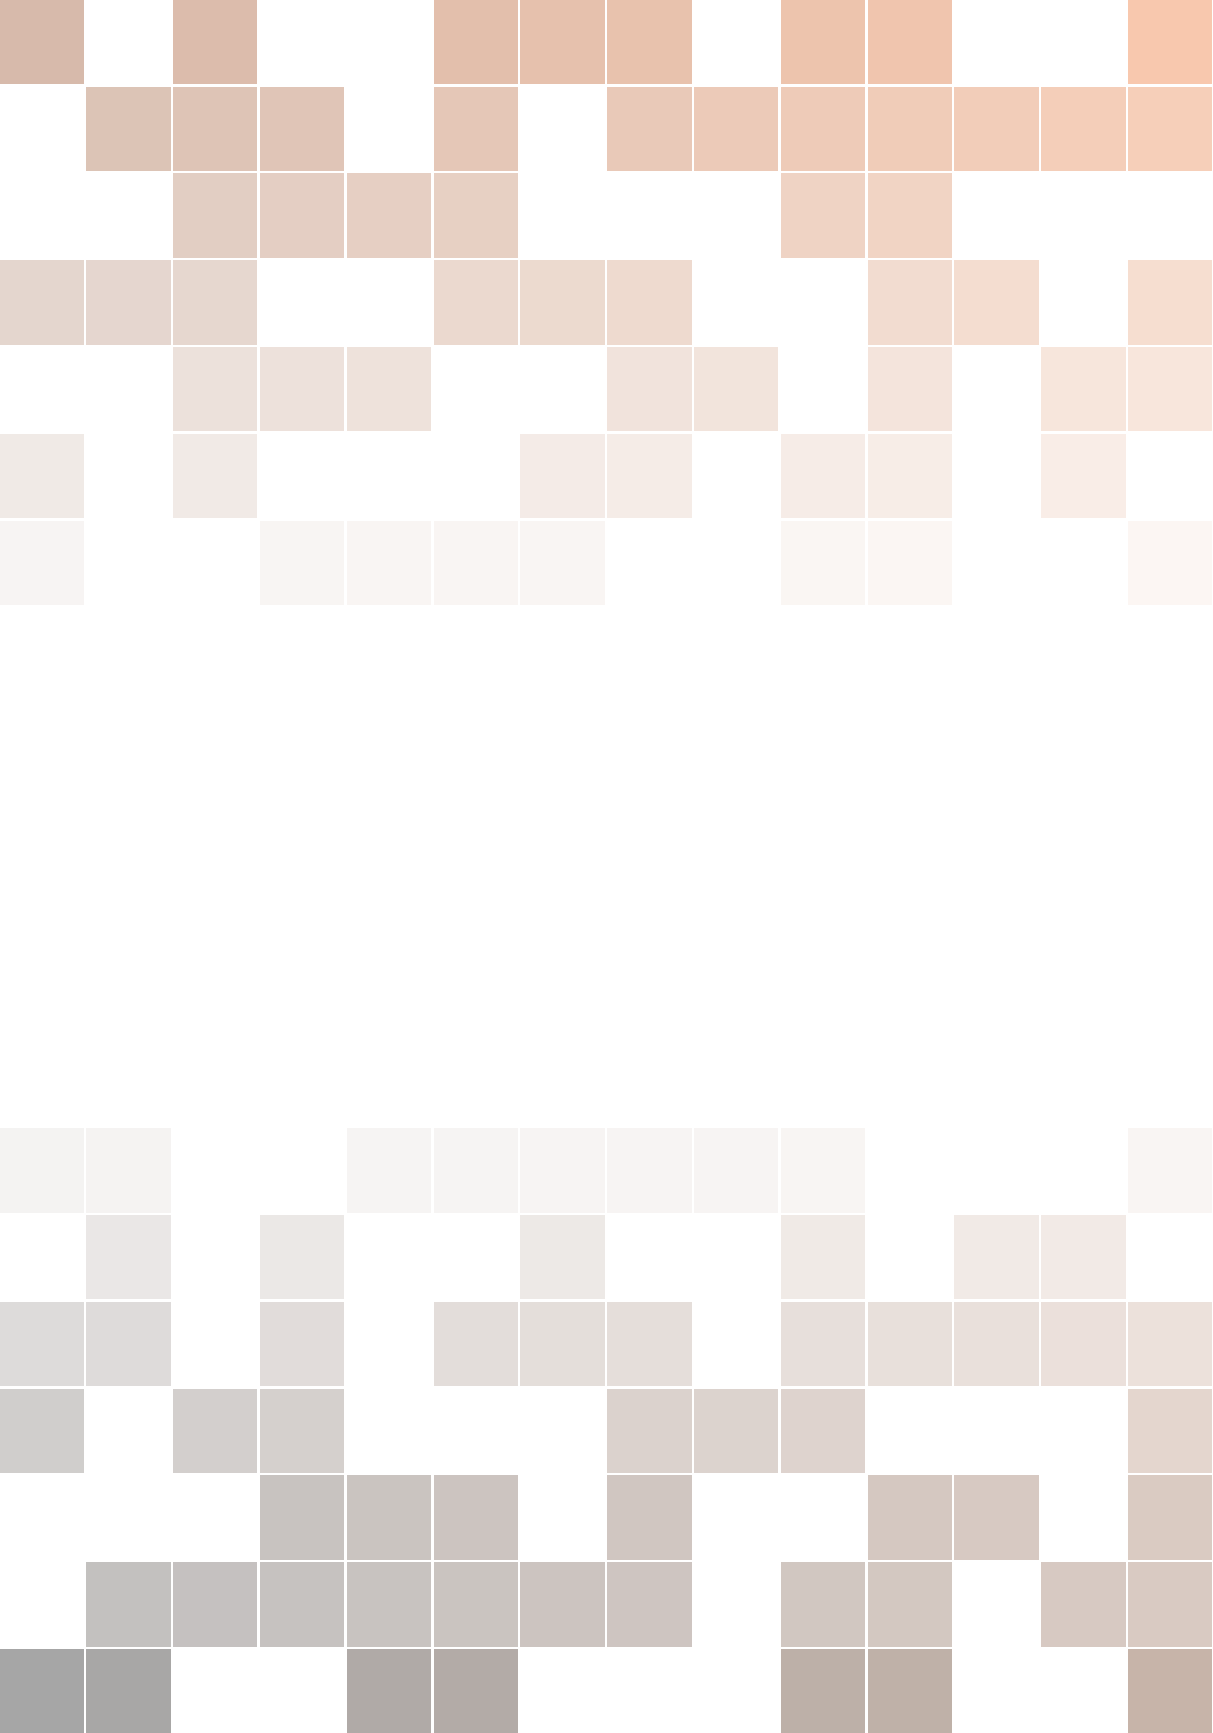
\includegraphics[width=\paperwidth]{images/background}}; % Background image
%\textsl{}
%      \draw[anchor=north] (midpoint) node [fill=ocre!30!white,fill opacity=0.6,text opacity=1,inner sep=1cm]{\Huge\centering\bfseries\sffamily\parbox[c][][t]{\paperwidth}{\centering Coding Interview Essentials\\[15pt] % Book title
%      {\Large - }\\[20pt] % Subtitle
%      {\huge Davide Spataro}}}; % Author name
%    \end{tikzpicture}};
%\end{tikzpicture}
%\vfill
%\endgroup


\includepdf[pages={2},fitpaper=true]{images/book_covers1.pdf}


	%\usechapterimagefalse % If you don't want to include a chapter image, use this to toggle images off - it can be enabled later with \usechapterimagetrue

	\chapterimage{images/header} % Table of contents heading image
	
	\pagestyle{empty} % No headers
	
	\tableofcontents % Print the table of contents itself
	
	%\cleardoublepage % Forces the first chapter to start on an odd page so it's on the right
	
	\pagestyle{fancy} % Print headers again
	

	%!TEX root = ../main.tex
%%%%%%%%%%%%%%%%%%%%%%%%%%%%%%%%%%
% Links:
%
% Difficulty: Easy/Medium Companies: 
%%%%%%%%%%%%%%%%%%%%%%%%%%%%%%%%%%

%\chapterimage{header}

\chapter{Power set generation}
\label{ch:power_set}
\section*{Introduction}
The concept of power set is familiar to many because it is introduced very early during
introductionary math courses on set theory. The problem described in this chapter is about writing
an algorithm that is capable of finding the powerset of a given set. Two main solution approach are
presented here, one that is strightforward deriving immediately from the recursive definition of
power set\footnote{The following is the recursive definition of powerset. In words the powerset of an empty
set is a set contains as only element the empty set itself. For a non-empty set, let $e$ be an
element of the set and T be the original set minus $e$ (relative complement). The powerset can
be then definied as the union of two distinct powersets. The powerset of T (all the subsets not
containing $e$) and the powerset of T modified in a way such that $e$ is added to all of its
element.
\begin{equation}
	\mathcal{P}(S)=\begin{cases} 
\{\{\}\} & \text{if } P=\{\} \\
P\{T\} \bigcup \{t \in P\{T\} : t \cup \{e\}\} \text{ where } e \in P, \text{ and } T = P \setminus \{e\} & \text{otherwise}
\end{cases}
\label{eq:power_set_recursive_definition}
\end{equation} 
} (See Equation \ref{eq:power_set_recursive_definition}), while the other is based on a clever
observation about the distribution of the bits among the integers from $0$ to the size of the
powerset. The problem is usually presented in a very direct manner with a short and concise
statement because the interviewer is expecting the candidate to be already familiar with the
concept.



\section{Problem statement}
	\begin{exercise}
		Write a function that given a set of elements $P$ returns its power-set. A power-set of a set $P$,
		(here denoted as $\mathcal{P}(S)$ is the set of all its subsets including the empty subset
		$\emptyset$ and $P$ itself.

		\begin{example}
			\hfill \\
			For example, given the set $P=\{a,b,c\}$, the following two sets are both correct outputs for
			this problem:
			\begin{equation*}
				\{\{\}, \{b,c\}, \{a\}, \{a,b\}, \{a,b,c\}, \{b\}, \{a,c\}, \{c\} \}
			\end{equation*}
			\begin{equation*}
				\{\{\}, \{a\}, \{b\}, \{c\}, \{a,b\}, \{b,c\}, \{a,c\}, \{a,b,c\} \}
			\end{equation*}
			
		\end{example}
	\end{exercise}
\section{Clarification Questions}

\begin{QandA}
	\item What is the maximum size of the input?
	\begin{answered}
		\textit{The maximum number of element is strictly less than $n < 32$.}
	\end{answered}
	
	\item Are all the element in the collection distinct?
	\begin{answered}
		\textit{No, the elements are not necessarily distinct. $S$ can contain duplicates.}
	\end{answered}

	\item Can the subset in the power-set appear in any order?
	\begin{answered}
		\textit{Yes, subsets can appear in any order.}
	\end{answered}
\end{QandA}

\section{Discussion}
\label{sec:powerset:discussion}
There is one key point that should immediately be noticed: \textbf{The powerset of a collection of
	$n$ elements has size} $\boxed{2^n}$\footnote{The proof of this fact is relatively easy and it boils
	down to the fact that a subset of $P$ is basically $P$ with possibly some of the elements
	removed from it. Because we two possible choices we can make for every element of $S$ (either
	remove or not remove and element) then the total number of possible subset is: $2 \times 2
	\times \ldots \times 2 = 2^{|P|}$. Two choices for the first element, two for the second, and so
	on until the last element of $P$.} . This fact should be immediately pointed out during the
	interview, stressing the fact that the constraint $n < 32$ is a strong hint towards the fact
	that an exponential solution is expected. After-all we are required to output all the elements
	of the powerset, and thus the complexity of any algorithm solving this problem cannot be less
	than the size of the powerset itself. Doing so shows general knowledge on set theory and the
	ability to link and use that knowledge with the problem statement.


\subsection{Backtracking}
The first solution presented in this chapter is based on the fact that that during the generation of
one of the elements of the power-set a decision has to be taken for each element of the original
set, on whether to include the element or not into the subset. When a decision for the first element
is taken then what we are left with is $|P|-1$ decisions before we have created a valid subset of
$|P|$. 
This kind of process can be easily visualized with a tree where a node at level $i$
represents a decision for the $i^{th}$ element and a path from the root to a leaf uniquely
identifies a subset of $P$ i.e. $n$ decisions. 
All paths from the root to the leafs thus, represent the power set. In
order to solve this problem we have to explore the entirety of this tree. An example of such tree is
shown in Figure \ref{ref:power_set_decision_trees}.

One general way to deal with such type of problems is by using backtracking to try all possible
decision paths for each of the elements. The general idea is that we are going to, for all elements
starting from the first until the last, to explore the two possibilities: take or exclude the
element from the subset. Backtracking is a general algorithm that allows to enumerate and explore
large search spaces like this one. The main idea is that we first try to stick with a decision for
the first element, and we continue from there to generate all possible subsets where said decision
is never changed. When there is no more subset to generate, we backtrack and change our first
decisions to the next possible one and repeat the process of generating all possible subsets.
The proposed solution will incrementally construct one subset at the time, using an integer variable
to keep track of which element we are currently
deciding to include or exclude. The base case of the recursion happen when there is no more decision
to take, meaning that the current subset is ready to be included in the solution (it has been
produced after $n$ decision steps).

The C++ code implementing the idea above is shown in Listing \ref{list:power_set_backtracking}. The
complexity of this solution is exponential i.e. $O(2^n)$ which as already pointed out is as good as
it gets.


	\lstinputlisting[language=c++, caption="C++ to the power set generation using backtracking",label=list:power_set_backtracking]{sources/power_set/power_set_backtracking.cpp}


\begin{figure}
	\centering
	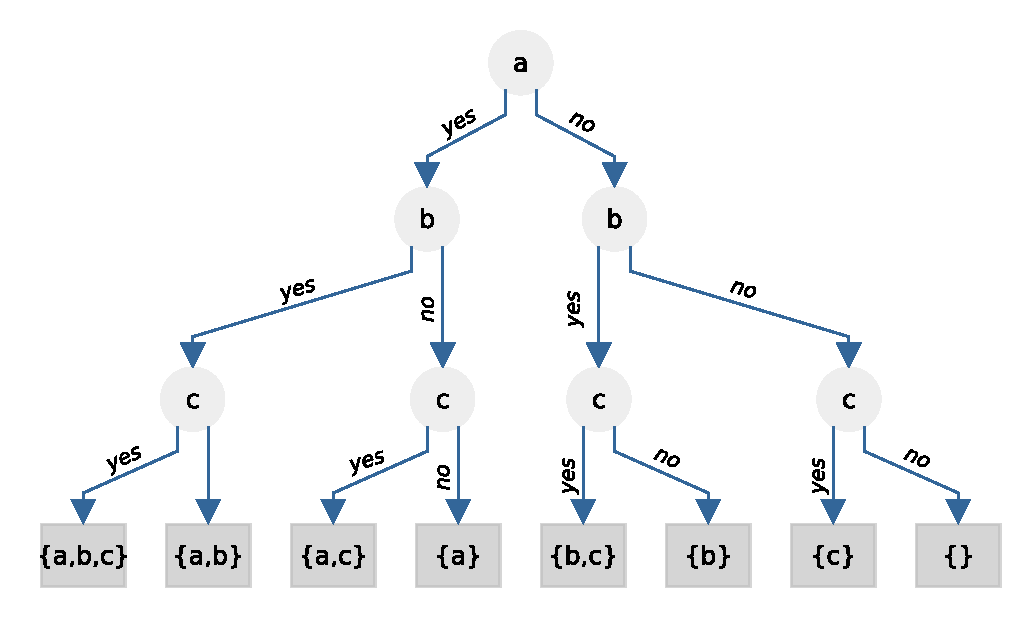
\includegraphics[width=\textwidth]{sources/power_set/images/tree}
	\caption[Decision tree for the power-set generation using backtracking.]{Decision tree for the power-set generation using backtracking. At level $i$ are the decision for the element $i$ in the original set. A labal marked with yes identifies the decision to take the corrensponding element into the subset, while a node labeled with no the opposite. At the last level is the powerset.}
	\label{ref:power_set_decision_trees}
\end{figure}

The advantages of using the backtracking framework to solve this problem is that, once we notice
that this problem can be solved by fully exploring the search tree, then we can immediately
start writing the code and rely on our experience as backtracking algorithm writers to implement a correct
solution with the added bonuses of being concise and short when written in a recusive form  as well
as well understood.
The downside is that the iterative implementation can be a little harder and more verbose to write.
Regardless of which one you choose, the interviewer is going to be pleased with your code provided you get to the final solution
without making too many implementation mistakes (forgetting to add the base case, or coding it wrong
is a pretty common one).

\subsection{Bit Manipulation}
Another approach that can be used to solve this problem is based on the fact that the values of the
bits of the numbers $\{0,1,2,\ldots, s^n-1\}$  already provide all the information necessary to make
the decision weather to include or not an element from the original set. 
The main idea is that the binary representation of the numbers from $0$ to $2^{n}-1$ is basically
the powerset of $n$ bits.
In other words, the binary representation of any of those numbers can be used to build one subset out
of the $n$ elements of the input set. 
For instance given the input $S=\{a,b,c\}$ the Table \ref{tab:mapping_value_bits} shows numbers from $0$ to $2^3-1 = 8$ and their bit
representation (second column) and how such information about which bit is set or not can be used to construct one
subset of the power-set of $P$ (third column). When the $i^{th}$ bit is set i.e. its value it $1$, it means that
corresponding $i^{th}$ element of $P$ is taken, while a non-set bit (with value $0$) means it is
excluded.

\begin{table}
	\centering
	\begin{tabular}{|l|l|l|}
		\hline
		Value & Bits & Subset\\ \hline
		0     & 000  & $\{\}$\\ \hline
		1     & 001  & $\{c\}$\\ \hline
		2     & 010  & $\{b\}$\\ \hline
		3     & 011  & $\{b,c\}$\\ \hline
		4     & 100  & $\{a\}$\\ \hline
		5     & 101  & $\{a,c\}$\\ \hline
		6     & 110  & $\{a,b\}$\\ \hline
		7     & 111  & $\{a,b,c\}$ \\ \hline
	\end{tabular}
	\caption[Mapping between bits and element of the powerset.]{This table shows a 1-to-1 mapping between integer values, their binary representation and an element of the powerset.}
	\label{tab:mapping_value_bits}
\end{table}

This idea can be used to write an algorithm in which all the numbers in the range $\{0,1,2,\ldots,
s^n-1\}$ are considered and each of them is used to generate a subset of the final solution.
Basically every number from such range maps uniquely to a subset of the powerset. It is really not
surprising when we think about the meaning of a bit in the binary representation of integers. One
can build a number by summing up powers of $2$ and the bits contains the information on whether a
certain power of two should be added to the final value for the represented number or not. With $n$
bits one can represents $2^n$ numbers, each corrensponding to one subset of the powerset of those
$n$ bits.

Listing \ref{list:power_set_bits} shows  a possible C++ implementation of the idea above\footnote{Notice the usage of the \texttt{reserve}
function that should be used in all those scenario when we already know the final size of the
collection we are building. This saves times because avoids intermediate allocation and copy that
must happen during the resize of the vector.}. The complexity of this implementation is, not
surprisingly, $O(2^n)$\footnote{Not considering the constant price of $32$ that we pay for each
subset generation due to the fact that we need to inspect the value of all of the bits}. Also please
pay attention to the fact that the proposed implementation assumes that the size of
\lstinline[columns=fixed]{int} is $4$ bytes, which is true for most architecture but not for all\cite{cit::std::fundamentaltypes}. A better
implementation would use \lstinline[columns=fixed]{std::numeric_limits<int>::digits} instead of
the magic number $32$.



	\lstinputlisting[language=c++, caption="C++ backtracking solution to the problem of generating the powerset.",label=list:power_set_bits]{sources/power_set/power_set_bit_manipulation.cpp}


%\section{Common variations}

%\section{Conclusion}

	%!TEX root = ../main.tex
%%%%%%%%%%%%%%%%%%%%%%%%%%%%%%%%%%
% Links:
%
% Difficulty: Easy/Medium
% Companies: 
%%%%%%%%%%%%%%%%%%%%%%%%%%%%%%%%%%

\chapterimage{header}

\chapter{Square root of an integer}
\label{ch:square_root}
\section*{Introduction}
Calculation of the square root of an integer is a problem that is very often asked in coding interview question mostly because there exists a quite obvious solution that is not trivial to implement and a faster solution that works for larger input. It is a very good question to showcase implementation skills and algorithmic thinking.

\section{Problem statement}
Write a function (with signature: \lstinline[columns=fixed]{int my_sqrt(const int n)} ) calculates the square root of an integer rounded down to the nearest integer without using any library call.

\begin{example}
	\hfill \\
	\begin{itemize}
		\item[-] 	\lstinline[columns=fixed]{my_sqrt(9)=3}: $\Longleftarrow $ $\ceil{\sqrt{9}}=3$
		\item[-] 	\lstinline[columns=fixed]{my_sqrt(11)=3}: $\Longleftarrow $ $\ceil{\sqrt{11}}\approx\ceil{3.316624}=3$
		\item[-] 	\lstinline[columns=fixed]{my_sqrt(18)=4}: $\Longleftarrow $ $\ceil{\sqrt{11}}\approx\ceil{4.242640}=4$
	\end{itemize}

\end{example}

\section{Clarification Questions}

\begin{QandA}
	\item What is the maximum value the parameter $n$ can take?
	\begin{answered}
		\textit{The maximum number of element smaller than $2^{32}$.}
	\end{answered}
	
	\item Is $n$ guaranteed to be always positive?
	\begin{answered}
		\textit{Yes, there is no need to check for invalid input.}
	\end{answered}
\end{QandA}

\section{Discussion}
The interviewer is very likely expecting to see a brute force solution appear on the whiteboard within the first 5-7 minutes. The reason is that the brute force approach for this problem is quite easy conceptually but its implementation in a concise manner requires some thinking. 

\subsection{Brute-Force}
The square root of a number can be found by testing all numbers from $k=0,1,2,\ldots$ until a solution is found i.e. $k^2\leq n$ and $(k+1)(k+1) > n$ . A solution is guaranteed to be found, and it should be immediately noticed that no more than $\sqrt{n}$ numbers will be tested. Therefore the time complexity of this approach is $O(\sqrt{n})$.
Listing \ref{list:square_root_brute_force} shows a possible implementation. Note that the variable $i$ has a type in C++ that is larger in size than $int$. This prevents overflows during the calculation of $i^2$ in the while condition if the input $n=2^{32}$.

\begin{minipage}{\linewidth}
	\lstinputlisting[language=c++, caption=$O(\sqrt{n})$ solution to the problem of finding the square root of an integer.,label=list:square_root_brute_force]{sources/square_root/square_root_brute_force.cpp}
\end{minipage}

\subsection{Logarithmic Solution}
Binary search can be effectively used to solve this problem. In order to show that, it is beneficial to look at the problem from a slightly different angle. 
Let 
\begin{equation}
	F(k)=\begin{cases} 
0 & k^2 \leq n \\
1 & k^2 > n
\end{cases}
\label{eq:square_root_piecewice}
\end{equation} 
be a piece-wise function that partition the search space $[0\ldots n]$ into two sets (See Table \ref{tab:sqrt_split_space}):
	\begin{itemize}
      \item [-] the numbers  less or equal than $\sqrt{n}$
      \item [-] the numbers strictly greater or equal than $\sqrt{n}$
	\end{itemize}

\begin{table}[]
	\centering
	\begin{tabular}{|c|c|c|c|c|c|c|}
		\hline
		$0$ & $1$ & $2$   & $\sqrt{n}$ & $\sqrt{n}+1$ & \ldots   & $n$ \\ \hline
		$0$ & $0$ & \ldots & $1$ & $1$ & \ldots & $1$   \\ \hline
	\end{tabular}
\label{tab:sqrt_split_space}
\caption{Partition of the search space according to the function in Eq. \ref{eq:square_root_piecewice}}
\end{table}
What the function should return is basically the greatest $k$ s.t. $F(k)=0$. 

Because of the peculiarity of the function $F(k)$ i.e. (divided into two partition) we can use binary search to find the end of the first partition as shown in Listing \ref{list:square_root_binary_search}. Note how a the algorithm works by iteratively searching in a smaller subinterval defined by the variables $l$ and $r$. At each iteration test the middle element of the subinterval (variable $middle$), and this can lead to three scenarios:

\begin{enumerate}
 	\item $(middle)^2  = n \longrightarrow$. $middle$ is the solution. $n$ is a perfect square and $\sqrt(n)=middle$
 	\item $(middle)^2  > n \longrightarrow$. $middle$ is not the solution and we can also exclude all numbers $k \geq middle$ (by doing $r = middle-1$).
 	\item $(middle)^2  < n \longrightarrow$. $middle$ is the best guess we have found so far. we can also exclude all numbers $k < middle$ from the next iterations (by doing $l = middle+1$).
\end{enumerate}
As a bonus it might be also good to point out to the interviewer the fact that the middle element is not calculated as it is commonly done i.e. $(l+r)/2$ in order to prevent overflow when $l+r$ is calculated.

\begin{minipage}{\linewidth}

	\lstinputlisting[language=c++, caption=$O(log_2(n))$ solution to the problem of finding the square root of an integer.,label=list:square_root_binary_search]{sources/square_root/square_root_binary_search.cpp}
\end{minipage}

Not surprisingly the complexity of this solution is logarithmic.


\section{Conclusion}

	%!TEX root = ../main.tex
%%%%%%%%%%%%%%%%%%%%%%%%%%%%%%%%%%
% Links:
%
% Difficulty: Easy/Medium Companies: 
%%%%%%%%%%%%%%%%%%%%%%%%%%%%%%%%%%

\chapterimage{header}

\chapter{Two string anagram}
\label{ch:two_string_anagram}
\section*{Introduction}
From a set of words, you can construct other words by only changing the arrangements of their characters.
For instance, from the characters in \textit{"alerting"} you can spell the following words:
\begin{itemize}
	\item  \textit{"altering"}
	\item  \textit{"integral"}
	\item  \textit{"relating"}
	\item  \textit{"triangle"}.
\end{itemize}
Words sharing the same characters set are called \textbf{anagrams}. 

Being able to create good anagrams, especially if they are able to reflect or comments on the words they are generated from (for instance turning
\textit{"Madam Curie"} into \textit{"Radium came"}) is regarded as a rather difficult task.
Computers have been used for a long time to find anagrams in long texts, as well as to generate the so-called anagram dictionaries.  A special kind of dictionary, where all the letters in a word and
all their transposition are arranged in alphabetical order,  are often used in games like
Scrabble\footnote{https://en.wikipedia.org/wiki/Scrabble}. Often, at the core of such applications lies an efficient algorithm for determining if a word is an anagram of another word.

As it is pretty clear at this point, the problem discussed in this lesson is about anagrams, and more specifically, about determining the number of
modifications you need to make to a word in order to make it a valid anagram of a
another word.
This kind of question is considered rather easy during a coding interview process, as it does not require particular insights or particularly tricky reasoning in order to come up with an efficient solution, aside from understanding the concept of an anagram, which is common knowledge.

That said, it is still very much worth studying this problem as it is frequently asked during the preliminary interview stages. Moreover, despite its simplicity, there is more than one neat and elegant approach leading to an efficient
solution to this problem.

In the rest of the chapter we are going to have a look at three
solutions, starting from the slow but easy to understand brute-force in Section \ref{sec:anagrams:bruteforce} then touching briefly on a faster approach using sorting in Section \ref{sec:anagrams:sorting},and finally, and finally, we will get to the optimal solution running in linear time in Section
\ref{sec:anagrams:histograms}. 

\section{Problem statement}
	\begin{exercise}
		Write a function that given two string, $a$ and $b$ of length $n$ and $m$, respectively, determines the minimum number of character substitution, $C(s, i, c)$, necessary to make the string $a$ an anagram of the string $b$.

		Two strings are said to be anagrams of one another if you can turn the first string into the second by rearranging its letters. 

		A substitution operation $C(s,i,c)$ modifies the string $s$, by changing its $i^{th}$ character into $c$. Notice that deletions or additions of characters are not allowed.
		The only operation you can do is change a character of the first string into another one. 

		In other words, what is the minimum number of characters of the input strings that need to be modified (no addition or deletion)  so that $a$ becomes an anagram of $b$?
		
	\begin{example}
		\label{ex:two_string_anagram:example1}
		\hfill \\
		\begin{itemize}
			\item 	a = "aaa"
			\item 	b = "bbb"
		\end{itemize}
		The function returns $3$. 
		All the characters of \textit{a} need to be changed into \textit{'b'}.
		\label{ex:anagrams:example1}
	\end{example}

	\begin{example}
		\hfill \\
		\begin{itemize}
			\item 	a = "tear"
			\item	b = "fear"
		\end{itemize}
		The function returns $1$. 
		All it is necessary is turning the first letter \textit{'t'} into a \textit{'f'}.
	\end{example}

	\begin{example}
		\hfill \\
		\begin{itemize}
			\item[] 	a = "Protectional"
			\item[] 	b = "Lactoprotein"
		\end{itemize}
		The answer for this case is $0$ because \emph{Protectional} is already an angram of \emph{Lactoprotein}.
	\end{example}
\end{exercise}

\section{Clarification Questions}

\begin{QandA}
	\item \begin{questionitem} \begin{question} Are the letters of the string always only letters from the English alphabet?    \end{question}      
    \begin{answered}
		\textit{Yes, letters are always from the English alphabet.}
	\end{answered} \end{questionitem}
	
	\item \begin{questionitem} \begin{question} Should the function be case sensitive?   \end{question}      
    \begin{answered}
		\textit{ No. You can assume the input letters are always lower case.}
	\end{answered} \end{questionitem}
	\item \begin{questionitem} \begin{question} Can the input string be modified? No, the input is immutable.  \end{question}      
    \begin{answered}
		\textit{No, the input strings are immutable.}
	\end{answered} \end{questionitem}

	\item \begin{questionitem} \begin{question} What value should be returned when there is no solution?  \end{question}      
    \begin{answered}
		\textit{In such case you can return $-1$.}
	\end{answered} \end{questionitem}
\end{QandA}

\section{Discussion}

Let's start by first quickly review what the word anagram means in the context of this problem. First of all, notice that both $a$ and $b$ contain a single word (which can be fairly long).
Moreover, for $a$ to be an anagram
of $b$, it has to be the case that exists an arrangement of characters in $a$ that is equal to $b$.
In other words, the question to which we need to answer is: is it possible to shuffle the character of $a$ such that we obtain $b$?
For this to be the case, it must be that $a$ and $b$ contain the same set of characters meaning that sorting both $a$ and $b$ would make them equal.
In addition, as a consequence of the fact that no addition or deletion
is allowed, \textbf{$a$ and $b$ must have the same length}. 
On the other hand, if they have the same length then it is always
possible to solve this problem because in the worst case, we can modify every letter of $a$ (see Example \ref{ex:two_string_anagram:example1}).
Thus, the only case when the problem has no solution has been isolated: when $n \neq m$ we must return $-1$ otherwise we can proceed with our calculation knowing that a solution exists.

\subsection{Brute-Force}
\label{sec:anagrams:bruteforce}
One of the first options coming to mind is a solution where we generate all possible arrangements of the letters in $a$, and for each of these arrangements, calculate the number of modifications necessary to convert it into $b$. 
The key idea is that the cost of transforming a string into another is equal to the number positions having different letters. 
For instance, the cost of transforming \textit{"abcb"} into \textit{"bbbb"} is $2$ because the two strings differ in the first and third letters. 

Although it is simple to explain, this approach must be considered poor because the number of arrangements of a set of $n$ letters grows as fast as $n!$.
Moreover, enumerating all the arrangements is no trivial task, unless we use a  library function capable of doing that (for instance, the C++ standard library provides the function \inline{std::next_permutation}\footnote{\href{https://en.cppreference.com/w/cpp/algorithm/next_permutation}{https://en.cppreference.com/w/cpp/algorithm/next\_permutation}} devoted to this purpose).


Listings \ref{list:two_string_anagram_bruteforce} shows a C++ implementation of the idea above.

\lstinputlisting[language=c++, caption="Brute force.",label=list:two_string_anagram_bruteforce]{sources/two_string_anagram/two_string_anagram_brute_force.cpp}


\subsection{Sorting}
\label{sec:anagrams:sorting}
The brute-force solution does a lot of superfluous work, because it tries to find a permutation of the string $a$ requiring minimal modifications to be morphed into $b$.
But is it really necessary to turn $a$ into \textbf{exactly} $b$, or is it sufficient to modify $a$ so that it is equal to a particular permutation of $b$? 
After all, being an anagram is a transitive property: if $a$ is a permutation of $b$ and $b$ is a permutation of $c$, then $a$ must also be a permutation of $c$. 

By definition, an anagram of $b$ is any permutation of its characters, and therefore, the particular permutation in which the characters of $b$ are sorted is a valid anagram on its own. 
It is much easier than checking all possible permutations, to modify $a$ into the "sorted" anagram of $b$ (where all of its characters are sorted), rather than to exactly $b$ because all we need to do is to create a copy of both $a$ and $b$, sort both of them and then calculate the character-by-character difference.
\textbf{This approach works because if $x$ is an anagram of $b$ then $x$ is also an
anagram of `sort(b)`}.
In other words, it does not matter how the characters are arranged in $a$ and $b$, as the only thing that matters is the set of the characters
appearing in $a$ and $b$: the order in which characters in both $a$ and $b$ appear does not matter. 

Listings \ref{list:two_string_anagram_sorting}  shows how we can take advantage of this fact and write a fast solution for this problem.

\lstinputlisting[language=c++, caption="Solution based on sorting.",label=list:two_string_anagram_sorting]{sources/two_string_anagram/two_string_anagram_sorting.cpp}

Notice that, if the input was mutable, then, the additional space occupied by the copies of the string \inline{aa} and \inline{bb} could have been avoided. 

The time complexity of Listing \ref{list:two_string_anagram_sorting}  is $O(n log(n))$ (because of sorting). The space complexity is $O(n)$ (we create copies of the input strings).



\subsection{Histograms}
\label{sec:anagrams:histograms}


There is another bit of information that we have not used yet: \textbf{the alphabet} from which the
letters of $a$ and $ab$ are taken from \textbf{is small}. 
If the only thing that matters is the set of characters appearing in $a$ and $b$ (and not their order, as discussed above),
then we can use the same idea at the core of the \href{https://en.wikipedia.org/wiki/Bucket_sort}{bucket sort} algorithm to achieve a linear time complexity solution.


The key idea is to pre-process $a$ and $b$ so to calculate their per-character frequencies, denoted here as $F_a$ and $F_b$, respectively.
An entry of $F_a[\mathrm{c}]$ and $F_b[\mathrm{c}]$, where $\mathrm{c} \in \{\mathrm{a},\mathrm{b},\ldots,\mathrm{z}\}$ (a letter of the alphabet), contains the frequency of character $\mathrm{c}$, in $a$ and $b$, respectively.


If $F_a$ and $F_b$ are the same, then $a$ and $b$ have exactly the same character set and $a$ is an anagram of $b$.
Otherwise, it must be the case that some characters of $a$ appear in $b$ a different number of times.
In this case, we can fix $a$ in such a way to make sure that its frequencies $F_a$ ey match the ones in $F_b$. 
But the main question is still unanswered: how many operations are necessary to do so?  In order to get this answer, it is useful to look at
the difference ($D$) of $F_a$ and $F_b$.

$D = F_a - F_b = \{D[\mathrm{a}] = (F_a[\mathrm{a}] - F_b[\mathrm{a}]), D[\mathrm{b}] = (F_a[\mathrm{b}] - F_b[\mathrm{b}]), D[\mathrm{c}] = (F_a[\mathrm{c}] - F_b[\mathrm{c}]), \ldots, D[\mathrm{z}] = (F_a[\mathrm{z}] - F_b[\mathrm{z}])\}
$

$D[\mathrm{c}]$ (where $\mathrm{c} \in \{\mathrm{a},\mathrm{b},\ldots,\mathrm{z}\}$) contains the difference between the number of occurrences of the character $\mathrm{c}$ in the string $a$ and $b$. Depending on whether the value of $D[\mathrm{c}]$  is greater or smaller than $0$, $a$ has an excess or a deficit of the letter c, respectively.

Firstly, notice that $\sum_{c=\mathrm{a}}^{\mathrm{z}} D[\mathrm{c}] = 0$. This observation stems from the fact that $|a|=n=m=|b|$ ($a$ and $b$ must have equal length for this problem to have a solution, remember?) and that if $a$ has an excess of a certain character $\mathrm{c}$ then there must exist another character $\mathrm{d} \neq \mathrm{c}$ that the string $a$ has a shortage of. If that is not the case, it is impossible for $a$ and $b$ to have equal length.

We can use this fact to modify the excesses of the letters of $a$, the ones having a positive value of $D$ into some of the letters there is a shortage of so that eventually, every single value of $D$ is zero.
If $D[\mathrm{c}] = x$ is going to take $x$ modifications to transform the excess of characters $\mathrm{c}$.
The answer to this problem is, therefore, the sum of all the positive numbers of $D$. 

Listings \ref{list:two_string_anagram_histogram} shows a possible implemenetation of the idea above.

\lstinputlisting[language=c++, caption="C++ solution to the two string anagram problem using the histogram approach.",label=list:two_string_anagram_histogram]{sources/two_string_anagram/two_string_anagram_histogram.cpp}

Notice how the array of differences of frequencies $D$ can be easily calculated without explicitly
computing the frequencies for the characters of $a$ and $b$ but by simply adding $1$ to $D[\mathrm{c}]$ when the letter $\mathrm{c}$ appears in $a$
and subtracting $1$ when it does in $b$. 

The time and space complexity of the code above is $O(n)$ and $O(1)$ in space (we are using an array of $128$ integers regardless of the size of the input). We cannot do any better than this, as all characters in the input strings must be at least read once.



%\section{Conclusion}

	%!TEX root = ../main.tex
%%%%%%%%%%%%%%%%%%%%%%%%%%%%%%%%%%
% Links: https://www.geeksforgeeks.org/count-pairs-with-given-sum/
% https://algorithms.tutorialhorizon.com/given-an-array-and-a-number-k-check-for-pair-in-array-with-sum-as-k-in-onlgn/
% https://coderbyte.com/algorithm/two-sum-problem https://en.wikipedia.org/wiki/Subset_sum_problem
%
% Difficulty: Easy Companies: Microsoft, Amazon, Google
%%%%%%%%%%%%%%%%%%%%%%%%%%%%%%%%%%

\chapterimage{header} % Table of contents heading image

\chapter{Two numbers sum problem}
\label{ch:two_numbers_sum}
\section*{Introduction}
The problem described in this lesson is probably one of the most asked during coding interviews nowadays, mostly 
during the early online stages of the hiring process: the interviewer pretty much expects a candidate to be at least familiar with the problem or to have read it at some point during his preparation.

The problem is hard enough to require non-trivial insights in order to be able to write a non-trivial solution but, at the same time, it is not so hard that it would take you hours to come up with something meaningful to say or to write.

We will have a look at a number of solutions: First, we will start from the inefficient brute force approach (and we will later refine it into a fast and time-optimal one);
Then we will delve also into a radically different approach based on sorting; finally, we will condense the strengths of all the solutions investigated so far into a time and space optimal solution that we think would do better in an interview context. As we will see, the final solution is efficient and not terribly difficult to write and explain (which are fundamental aspects of every successful coding interview).


\section{Problem statement}

\begin{exercise}
	Write a function that takes an array of integers $A$ of size $n$ and an integer $T$, and returns \textbf{true} if the sum of any two distinct elements $I$ is equal to $T$, \textbf{false} otherwise.

	More formally: Given an array $=\{a_1,...,a_n\}$ and $T$, where $a_i, T \in
	\mathcal{N}$, return:
	\begin{itemize}
		\item  \textbf{true} if $\: \exists \;i,j \:\: i \neq j$ s.t. $a_i+a_j = T$
		\item  \textbf{false} otherwise
	\end{itemize}
	

	\begin{example}
	\hfill \\
		Given $A=\{9, 4, 17, 42, 36, -3 ,15\}$ and $T=14$, the function returns \textbf{true} because we can obtain $14$ by summing
		up together the elements $17$ and $-3$.
		If $T=17$ the answer is \textbf{false}.
	\end{example}

	\begin{example}
	\hfill \\
		Given $A=\{1,3,7\}$ and $T=8$, the function returns \textbf{true} because we can obtain $8$ by summing
		up together the elements $7$ and $1$. If $T=6$ the answer is \textbf{false}.
	\end{example}

\end{exercise}	


\section{Clarification Questions}
\begin{QandA}
	\item \begin{questionitem} \begin{question} Is the input array modifiable?  \end{question} 	 
    \begin{answered}
		\textit{Yes, the input array can be modified.}
	\end{answered} \end{questionitem}	
	\item \begin{questionitem} \begin{question} Are the integers guaranteed to be all positive or all negative?   \end{question} 	 
    \begin{answered}
		\textit{No, $A$ can contain positive or negative numbers.}
	\end{answered} \end{questionitem}
	\item \begin{questionitem} \begin{question} Are the values in $A$ guaranteed to be from a given range?  \end{question} 	 
    \begin{answered}
		\textit{No, the input is arbitrary. No assumption can be made on the magnitude of the elements of $A$.}
	\end{answered} \end{questionitem}
	\item \begin{questionitem} \begin{question} Can a pair be made from an element and itself?  \end{question} 	 
    \begin{answered}
		\textit{No, the pair's elements should be distinct. You cannot use the same element $a_i$ twice. You can however use two elements at indices $i$ and $j$ s.t. $i \neq j$ and $a_i=a_j$.}
	\end{answered} \end{questionitem}
	\item \begin{questionitem} \begin{question} Are all elements in the array unique?  \end{question} 	 
    \begin{answered}
		\textit{No, duplicates are allowed.}
	\end{answered} \end{questionitem}
	\item \begin{questionitem} \begin{question} Is the input sorted?  \end{question} 	 
    \begin{answered}
		\textit{No, the ordering of $A$ is arbitrary.}
	\end{answered} \end{questionitem}
	\item \begin{questionitem} \begin{question} Shall the function integer overflow be considered when performing the sum of two integers? Is it possible for two elements of $A$ to sum up to a value that does not fit in a standard \inline{int}?  \end{question} 	 
    \begin{answered}
		\textit{No, you do not need to worry about overflow.}
	\end{answered} \end{questionitem}
\end{QandA}


\section{Discussion}

%%%%%%%%%%%%%%%%%%%%%%%%%%%%%%%%%%%%%%%
%        quadratic solution
%%%%%%%%%%%%%%%%%%%%%%%%%%%%%%%%%%%%%%
\subsection{Brute-force}
\label{sec:two_numbers:bruteforce}

The brute force solution is fairly straightforward because it consists of a direct application of the formal problem statement. 
The solution space consists of all possible ordered pairs $(a_i,a_j)$, $i < j$. 
Two nested loops can be used to enumerate all those pairs, and, for each of them, we can check whether their sum is equal to $T$: if that is the case,
then   \textbf{true} can be immediately returned, otherwise, if we have checked every possible pair and none of them was good, then we can return  \textbf{false}.
You will find an a fomalization and an implementation of this idea in Algorithm \ref{algo:two_number_sum_bruteforce}
and Listing \ref{list:two_number_sum_bruteforce}), respectively.

\begin{algorithm}
	\SetAlgoLined \SetKwFunction{FMain}{solveQuadratic}
	
	\KwIn{$ A $ \tcp{An array $A$ of length $n$}} \KwIn{$ T $ \tcp{An integer $T$}}

	\Fn{\FMain{$A,T$}}{
	
		%\Output{true if two distinct element of $A$ sum to $T$}
		
		\For{$i\leftarrow 0$ \KwTo $n-1$} {\For{$j\leftarrow i+1$ \KwTo $n$} {\If{$a_i + a_j =
		T$}{\Return True \;}}} \Return False \;}\textbf{End Function}
	
		\caption{Two loops, quadratic solution to the question in Section \ref{ch:two_numbers_sum} }
		\label{algo:two_number_sum_bruteforce}
\end{algorithm}


\lstinputlisting[language=c++, caption="C++ solution of the two number sum problem with a brute force approach.",label=list:two_number_sum_bruteforce]{sources/two_numbers_sum/brute_force.cpp}

The time complexity of this solution is $O(n^2)$ because there is a quadratic number of
ordered pairs and in the worst case, we will look at \textbf{all} of them.

The number of iterations of the internal loop depends on the value of $i$ and
it is described by the function: $f(i) = n-i-1$. The total number of iteration the second
loop runs in the worst case is the the sum of $f(i)$ for all values of $i$: 
$\sum_{i=0}^{n-2} f(i) = (n-1) + (n-2) + (n-3) \ldots + 1 =\sum_{x=1}^{n-1} x= \frac{n(n-1)}{2} = O(n^2)$

The space complexity is $O(1)$.



\subsection{Hashing}
\label{sec:two_numbers:hashing}
The internal loop of the brute force solution above can be eliminated entirely with the help of a hash table.
The key insight is that if a solution exists involving $a_i$ then, it must the case that exists another element $a_j  = a_i-T$ with $i > j$. 

What this means in practice is that we can loop through $A$ one element at a time and keep track, in a lookup table, of all the elements seen so far, so that the lookup operation for the aforementioned element $a_j$ can be performed in constant time.

Algorithm \ref{algo:two_number_sum_hashset} and Listing \ref{list:two_number_sum_hashing} shows this idea in code.

%%%%%%%%%%%%%%%%%%%%%%%%%%%%%%%%%%%%%%%
% two_numbers_sum_hashset       
%%%%%%%%%%%%%%%%%%%%%%%%%%%%%%%%%%%%%%
\begin{algorithm}
	%	\KwData{} \KwResult{Tr }
	\KwIn{$ A $ \tcp{An array $A$ of length $n$}} \KwIn{$ T $ \tcp{An integer $T$}} \KwOut{true if
	two distinct element of $A$ sum to $T$, False otherwise} \SetKwFunction{FMain}{solveHashSet}
	
    \Fn{\FMain{$A,T$}}{H $\longleftarrow$ \CreateHashSet \;
	
		\For{$i\leftarrow 0$ \KwTo $n$} {target $\leftarrow$ $(T-a_i)$ \eIf{H.find(target)} {\Return
		True} {H.insert($a_i$)}} \Return False\;}\textbf{End Function}

		\caption{Hashset, linear solution to the \textit{two number sum} question in Section
		\ref{ch:two_numbers_sum}.}
		\label{algo:two_number_sum_hashset}
\end{algorithm}


\lstinputlisting[language=c++, caption="C++ solution of the two number sum problem using hashing.",label=list:two_number_sum_hashing]{sources/two_numbers_sum/hashset.cpp}

The time complexity of this approach is $O(n)$ (technically is linear on average due to complexity of lookups in hash tables) because the input array is scanned once and for each
of its elements, only one lookup and insertion are performed in the hash table (both operations costing constant time on average).

The space complexity
is also $O(n)$, as in the worst case the whole input array is stored in the lookup table.

A common mistake when solving this problem using this approach is to insert the whole input array into the lookup table, and only after searching for $(T-a_i)$.
The mistake becomes evident when $T$ is an even number ($2 | T$) and $\frac{T}{2}$ appears in $A$  exactly once, at index $k$ i.e. $a_k = \frac{T}{2}$ causing \inline{H.find(T-a_k)} to return \textbf{true}, which is wrong because this corresponds to a solution where we sum $a_k$ twice to obtain $T$.

For instance, when $A=\{1,2,5,4\}$ and $T=10$ this approach wrongly returns \textbf{true}, even if there are not two elements at distinct indices in $A$ whose sum is $T$ (we would use $5$ twice to obtain $10$).
\begin{example}
	\hfill \\ 
	\begin{itemize}
		\item[] $A=\{1,2,5,4\}$
	\item[] $T = 10$
\end{itemize}
	Algorithm \ref{algo:two_numbers_sum_hashset_wrong} wrongly return true even if there are not two
	distinct elements whose sum is $10$.
\end{example}


%%%%%%%%%%%%%%%%%%%%%%%%%%%%%%%%%%%%%%%
% two_numbers_sum_hashset_wrong       
%%%%%%%%%%%%%%%%%%%%%%%%%%%%%%%%%%%%%%
\begin{algorithm}
	\SetKwInOut{Input}{input} \SetKwInOut{Output}{output}
	\SetKwFunction{CreateHashSet}{CreateHashSet<int>} \Input{An array $A$ of length $n$} \Input{An
	integer $T$} \Output{true if two distinct element of $A$ sum to $T$}
	
	\SetKwFunction{FMain}{solveHashSet} \Fn{\FMain{$A,T$}}{H $\longleftarrow$ \CreateHashSet \;
		\tcp{Add the whole array in the hashset}
		\For{$i\leftarrow 0$ \KwTo $n$} {H.insert($a_i$)\;}
		
		\For{$i\leftarrow 0$ \KwTo $n$} {target $\leftarrow$ $T-a_i$ \; \If{H.find(target)} {\Return
		True}} \Return False\;}\textbf{End Function}
		\caption{Hashset, linear solution to the \textit{two number sum} question in Section
		\label{algo:two_numbers_sum_hashset_wrong}
	\ref{ch:two_numbers_sum} }
\end{algorithm}


\subsection{Sorting and binary search}
\label{sect:two_number_problem_binary_search}

As with countless other problems on arrays, sorting the input often opens the
way to a faster and more efficient solution. 

We can start by asking ourselves how the problem changes if  $A$ is sorted. Sorted arrays are naturally associated with binary search, and for good reasons! Many problems can be solved efficiently by pairing sorting and binary search on arrays. 
This problem is not different, and we can use binary search if $A$ is sorted to substitute the internal loop of the brute force solution presented [above](). This way, we can  lower the overall complexity down to $O(n log(n))$; it costs
$O(n log(n))$ to sort the input array in the first place, and the actual search consists of $n$ binary
searches, each of them costing $O(log(n))$. 

The space complexity is $O(1)$ because no additional space is required, since the array is sorted in place.

Listing \ref{list:two_number_sum_sorting} shows a C++ implementation of this idea. Notice that it uses \inline{std::binary_search} from the C++ standard library and that a possible follow-up question might be to show your own version of the binary search algorithm.



\lstinputlisting[language=c++, caption="C++ solution of the two number sum problem with sorting and binary search.",label=list:two_number_sum_sorting]{sources/two_numbers_sum/two_numbers_sum_sorting.cpp}


\subsection{Sorting and two pointers technique}
\label{sec:two_numbers:twopointers}

There is a variation to the to the approach described in Section
\ref{sect:two_number_problem_binary_search} which still involves sorting but uses a two-pointers
technique instead of binary search to finish the job. 

The key idea is that once $A$ is sorted, the algorithm initializes
two pointers, one starting at the beginning ($p_s$) and the other at the end ($p_e$) of the array, respectively.
It continues by looking at the sum of the two elements pointed by the two pointers and moving one of
the two at each step using the following logic: 
\begin{itemize}
	\item if $a[p_s]+a[p_e] = T$ a solution has been found. The algorithm returns true.
	\item if $a[p_s]+a[p_e] > T$, $p_e=p_e-1$. The right pointer is moved to the left. 
	Moving	$p_e$ to the left has the effect of making the sum of the values pointed by the two pointers smaller (this has an effect at the next iteration). 
	\item if $a[p_s]+a[p_e] < T$, $p_s=p_s+1$. The right end pointer is moved to the left. Moving $p_s$ to the right has the effect of making the sum of the values pointed by the two pointers larger. 
\end{itemize}



Listing \ref{list:two_number_sum_two_pointers} shows an implementation of the idea above. Notice that compared to the solution using the binary search, this one is shorter and simpler to write. Moreover, it does not use library functions. 

\lstinputlisting[language=c++, caption="C++ solution of the two number sum problem with the two pointers tecnique.",label=list:two_number_sum_two_pointers]{sources/two_numbers_sum/two_numbers_sum_two_pointers.cpp}

Despite the overall time complexity is still $O(n log(n))$, this solution is likely to be faster than
the one using binary search, mostly due to the fact that the array is scanned linearly (which makes caches happier) by the two pointers and not in a scattered way as in the case of binary search.

%%%%%%%%%%%%%%%%%%%%%
\section{Common Variations}
\subsection{Four numbers sum problem}
\label{sec:four_number}

\subsection{Problem statement}

\begin{exercise}
Write a function that takes four arrays of integers, $A,B,C,D$ and a integer $T$,
and returns how many distinct tuple $(i,j,k,l)$ where exist such that $A_i+B_j+C_k+D_l = Y$.

\begin{example}
\hfill \\
Given:
	\begin{itemize}
		\item[-] 	$A=\{1,2\}$,
		\item[-] 	$B=\{-2,-1\}$,
		\item[-] 	$C=\{-1,2\}$,
		\item[-]	$D=\{0,2\}$, and 
		\item[-] 	$T = 0$
	\end{itemize}
The answer is $2$ because the only two valid tuples are:
\begin{enumerate}
	\item $(0,0,0,1)$: $A_0 + B_0 + C_0 + D_1 = 1 + (-2) + (-1) + 2 = T = 0$
	\item $(1,1,0,0)$: $A_1 + B_1 + C_0 + D_0 = 2 + (-1) + (-1) + (-1) = T = 0$
\end{enumerate}
\end{example}
\end{exercise}

\subsection{Na\"ive $O(n^4)$ solution}
We can solve this problem very easily by using the same approach we have described in Section \ref{sec:two_numbers:bruteforce}.
The idea is that we can use four nested loops and enumerate all possible 4-elements tuples of indices. Listing \ref{list:two_number_sum_naive} shows how such an idea can be implemented.
Goes without saying, that this is not the fastest solution we can come up with, considering it has a time complexity of $O(n^4)$

\lstinputlisting[language=c++, caption="Brute force na\"ive solution to the four numbers sum problem.",label=list:two_number_sum_naive]{sources/two_numbers_sum/variations/four_number_sum/four_number_sum_solution1.cpp}

Needless to say, that this is not the fastest solution we can come up with, considering it has a time complexity of $O(n^4)$.

\subsection{$O(n^3)$ solution}
The trivial solution shown in Listing \ref{list:two_number_sum_naive} can be improved by using a similar reason that lead us improve the brute-force 
quadratic time solution for the two numbers problem in Listing \ref{list:two_number_sum_bruteforce} to the linear time (and space) in Listing \ref{list:two_number_sum_hashing}.

The idea is that inner-most loop is searching for a value $D_l = x$  s.t. if it summed to $A_i+B_j+C_k$ gives us $T$; in other words: $x+(A_i+B_j+C_k)=T$.
Therefore $x = T-(A_i+B_j+C_k)$. If there is a way of avoiding a linear search in the array $D$ for such a value, then we could bring down the complexity from $O(n^4)$ to $O(n^3)$.

Thankfully, this is possible if we use a hash map. If we create a hashmap mapping the value of $D$ and to their frequencies, the inner-most loop of the $O(n^4)$ solution above can be substituted with a query to the hashmap which runs in constant time (on average). 

Listing \ref{list:two_number_sum_cubic} shows an implementation of such idea. 
Notice that, in order to obtain the maximum saving in terms of work avoided, the arrays are rearranged in such a way so that $D$ is the longest of the four input arrays. 

\lstinputlisting[language=c++, caption="Brute force cubic time solution to the four numbers sum problem.",label=list:two_number_sum_cubic]{sources/two_numbers_sum/variations/four_number_sum/four_number_sum_solution2.cpp}


\subsection{$O(n^2)$ solution using hashing}

This problem can be however be solved in quadratic time if we use hashmaps in a smarter way, to hold 
the frequencies of all the values we can obtain by summing up any two elements of $A$ and $B$ and of $C$ and $D$.
The key idea is that we can build two distinct hashmaps:
\begin{itemize}
	\item $AB$: holding the frequencies of the values obtainable by summing any two elements of $A$ and $B$
	\item $CD$: holding the frequencies of the values obtainable by summing any two elements of $C$ and $D$.
\end{itemize}

The space required for both $AB$ and $CD$ is quadratic, which is more than the space used by any of the previous solutions, but this extra space
enables us to solve this variation also in quadratic time. 

The idea is that we are going to spend $O(n^2)$ time to construct both $AB$ and $CD$
and then again $O(n^2)$ to calculate the final answer 
by searching into $CD$ for the value $T-y$ where $y$ is an element of $AB$. 
If such a value exists in $CD$ it means that there exists one element in  $A$ and one in $B$ such that they sum up to $y$ and
one element $C$ and one in $D$ such that they sum up to $T-y$. Summing all these elements up gives: $y+T-y = T$.
This approach is shown in Listing \ref{list:two_number_sum_quadratic}. 

\lstinputlisting[language=c++, caption="Quadratic time solution to the four numbers sum problem.",label=list:two_number_sum_quadratic]{sources/two_numbers_sum/variations/four_number_sum/four_number_sum_solution3.cpp}

Notice that the first thing we do is to fill $AB$ by looping over all possible pairs of elements from $A$ and $B$.
We then do the same thing for $CD$, and finally, in the last loop, we take care of calculating the answer by searching, for each element $(k,v)$ of $AB$, where $k$ is the sum obtained by one element of $A$ and one of $B$, and $v$ is the number of ways we can obtain it,
into $CD$ for the target value $T-k$. If such a value exists into $CD$ then we know we can obtain $T$. The number of times
that is possible is dictated by the frequencies of $k$ and of the target value in $CD$.

However, you might have already noticed that we do not really need to explicitly create the map $CD$. 
The idea is that when we create $CD$ we already have all the values of $AB$  and therefore for a given $C_i+D_j$ we can already find out how many pairs in $AB$ exists that we can use to get a total sum of $T$. 
This optimization does not really change the overall space complexity
but in practice this mean that we use half the memory and we avoid doing $O(n^2)$ work by eliminating the last loop.

Listing \ref{list:two_number_sum_quadratic_opti} shows this optimized version.


\lstinputlisting[language=c++, caption="Space optimized quadratic time solution to the four numbers sum problem.",label=list:two_number_sum_quadratic_opti]{sources/two_numbers_sum/variations/four_number_sum/four_number_sum_solution4.cpp}

	%!TEX root = ../main.tex
%%%%%%%%%%%%%%%%%%%%%%%%%%%%%%%%%%
% Links:
%
% Difficulty: Easy Companies: 
%%%%%%%%%%%%%%%%%%%%%%%%%%%%%%%%%%

\chapterimage{header}

\chapter{Unique Elements in a collection}
\label{ch:unique_elements}
\section*{Introduction}
I have to admit I was not really sure it was the case to write about a problem as easy as this one,
but I have seen it asked enough to think it is valuable to discuss how to attack and
code it well during an interview. 
The problem is about checking whether a string does not contain
duplicate characters and as we shall see it can be coded in a handful of lines. 
It is quite important that a candidate asks the right questions, 
as the interview might be really trying to ask
you an harder problem instead with some hidden constraints (for instance what if the charset is not
ASCII or groups of characters of the input string map to a certain element of a given alphabet),
and that the implementation is impeccable and efficient. 
As with most of the problems in
this book, there is usually a number of solutions ranging from easy and straightforward (and usually
suboptimal) to more complex and faster. This problem is no exeption.  We are going to have a look at 
a bruteforce approach in Section \ref{} while Section \ref{} will discuss a much faster solution using an approach 
that we believe is the one that should be used during a real interview.


\section{Problem statement}
Given a string $s$ of length $n$, return \textit{true} if it does \textbf{not} contains duplicate characters, \textit{false} otherwise. 

\begin{example}
\hfill
	\begin{itemize}
		\item [-] $s=$"graph" $ \longrightarrow$ \textit{true}
		\item [-] $s=$"tree" $ \longrightarrow$ \textit{false}
		\item [-] $s=$"Einstein" $ \longrightarrow$ \textit{false}
	\end{itemize}
	
\end{example}

\section{Clarification Questions}

\begin{QandA}
	\item What is the maximum size of the input?
	\begin{answered}
		\textit{The maximum length for the input string is $10^6$.}
	\end{answered}
	
	\item Are all character upper or lower case?
	\begin{answered}
		\textit{No, both upper and lower case might be present.}
	\end{answered}

	\item Is the function case sensitive?
	\begin{answered}
		\textit{Yes.}
	\end{answered}

	\item Can I assume characters only alphanumeric characters are present in the input?
	\begin{answered}
		\textit{Yes. ASCII upper and lower case latin letters and numbers only.}
	\end{answered}
\end{QandA}

\section{Discussion}
Being this problem so popular and simple, the interviewer is expecting you to come up
with a good solution in a relatively short time window. 
For this reason at least the obvious solution (shown in Section \ref{sec:unique_character:bruteforce})
should be immediately put on the table despite the fact it is probably not the most elegant and concise.

\subsection{Brute Force}
\ref{sec:unique_character:bruteforce}
One of the possible brute-force solutions to this problem works by looping
over each character of the input string $s_i$ once,
and for each of them checking if it is present in any of the subsequent position of $s$. 
In other word we check whether the following is true: $\exists \; j $ s.t.  $s_j=s_i \; j>i$.
A C++ implementation of this idea is shown in Listing \ref{list:unique_elements_brute_force1}. 
The code uses two simple nested loops to perform the checks where the internal loop has a
loop variable $j$ starting one position after $i$ as there is no need to check
all the values in the range $[0,i]$ as that work has been already performed during previous iterations. 

This solution works in $O(|s|^2)$ time and $O(1)$ space. 
It can be however, turned into a much faster solution (spoiler $O(1)$ time) using an idea that is at the core of the solution presented index
Section \ref{sec:unique_elements:constanttime}.

\begin{minipage}{\linewidth}
	\lstinputlisting[language=c++, caption="C++ solution for determining all characters in a string are unique.",label=list:unique_elements_brute_force1]{sources/unique_elements/unique_elements_brute_force.cpp}
\end{minipage}

Because what the inner loop is really doing is searching for the char $s[i]$ in a substring or $s$ string,  Listing
code shown in Listing \ref{list:unique_elements_brute_force1} can be made more expressive 
by substituting that loop with a call to the standard library \inline{find} function. Listing 
\ref{list:unique_elements_brute_force2} shows such version of the bruteforce solution which contains 
shorter and cleaner code, but also shows to the interviewer that you are
able to use the standard library and do not need to 
reinvent the wheel everytime an ubiquitous operation, like \texttt{find}, happends to be needed.
The complexity however remains unchanged.
\begin{minipage}{\linewidth}
	\lstinputlisting[language=c++, caption="C++ solution for determining all characters in a string are unique using \texttt{std::find}",label=list:unique_elements_brute_force2]{sources/unique_elements/unique_elements_brute_force_std.cpp}
\end{minipage}

\subsection{Linear Time}
\ref{sec:unique_elements:constanttime}
In Listing \ref{list:unique_elements_brute_force1} the internal loop is doing the hard work of
searching for a duplicate of the character at index $i$. By trading space for time we can improve the cost of that loop so that it runs in constant time.
The idea is that when we process the char $s[i]i$ all we need to do is check whether we have seen this character before.
However in order to be able to do that, everytime a character $i$ is processed we need to remember about it by for instance inserting it 
into an hashset.
If we do that then the search for the duplicate of $s[i]$ simply becomes a cheap hashset find query.
This idea is shown in Listing \ref{list:unique_elements_brute_force_map} which uses \inline{std::unordere_map} as hashset.
\begin{minipage}{\linewidth}
	\lstinputlisting[language=c++, caption="C++ solution for determining all characters in a string are unique in $O(n)$ using an hashset.",label=list:unique_elements_brute_force_map]{sources/unique_elements/unique_elements_brute_force_map.cpp}
\end{minipage}

This approach seems to effectively lower the time complexity down to linear (the outer loop apparently runs $O(|s|)$ times and the search query in $L$ costs $O(1)$\footnote{On average}),
but at the cost of some space. But how much space exactly? The intuition would say $n$ because that is the size of the
input string. But the string is made of characters from an alphabet $\Sigma$ which has a fixed (and rather small) size i.e. $128$ (the size of the ASCII table)
elements. 
The insert instruction will therefore not be executed more than $|\Sigma|$ times. Because of this the space complexity of this solution if
$O(1)$. 

\subsection{Constant time}
The previous argument can be expanded further more with the following idea: \textbf{every string
with more than $|\Sigma|$ character contains at least one duplicate}.
The key idea supporting this argument is that there is only a finite and fixed
number of unique characters in the alphabet of $|s|$ and therefore strings longer than the size of such charset must have duplicates. 
This is a consequence of the piegeonhole principle \footnote{\url{https://en.wikipedia.org/wiki/Pigeonhole_principle}}.
The longest string with only unique characters is one of the permutations of "abcde\ldots zABCD \ldots Z123 \ldots 9". 
Therefore, if $|s| > |\Sigma| = 128$ ($128$ is the size of the ASCII character set), we can immediately say that there 
is at least a duplicate in $s$ and return \inline{false}.
Thus the solution using the hashset has complexity of $O(1)$ because in the worst case after $|\Sigma|$
lookups the next one will be positive.
For this reason the checks can be limited to the first $|\Sigma|$ character. 
Note that this observation suddenly makes the brute force approach also $O(1)$
if $i$ and $j$ in Listing \ref{list:unique_elements_brute_force1} are forced to stay below
$|\Sigma|$.

Armed with these new arguments, the solution we suggest to present during the interview only uses a
stack allocated array of bool of size $|\Sigma|$ storing the information regarding the presence of a
character in the characters examined so far. If at any time the currenclty examined character has
been already seen, then there is a duplicate. See Listing
\ref{list:unique_elements_brute_force_final} for a possible implementation of this idea.

\begin{minipage}{\linewidth}
	\lstinputlisting[language=c++, caption="C++ solution for determining all characters in a string are unique in $O(n)$ using an hashset.",label=list:unique_elements_brute_force_final]{sources/unique_elements/unique_elements_brute_force_final.cpp}
\end{minipage}

\section{Conclusion}
	%!TEX root = ../main.tex
%%%%%%%%%%%%%%%%%%%%%%%%%%%%%%%%%%
% Links:
%
% Difficulty: Easy/Medium
% Companies: 
%%%%%%%%%%%%%%%%%%%%%%%%%%%%%%%%%%

\chapterimage{header}

\chapter{Greatest element on the right side}
\label{ch:greatest_right}
\section*{Introduction}
This chapter discusses a problem that is known for having been asked during on-site interviews at Amazon. 
It is a relatively easy problem on arrays where, in a nutshell, we are given one as input and we are asked to find for each element of its element the value of the largest element among the ones to its right. 

Since, as we shall see, it is not a particularly challenging problem as all the information to come up with a good solution are hiding in plain sight in its statement, it is essential to focus our efforts towards making a good impression on the interviewer by showing clean reasoning, clear and simple communication as well as an elegant implementation of the solution.



\section{Problem statement}
\begin{exercise}
You are given an array $A$ of size $n$. You have to modify $A$ in place s.t. $A[i] = max(A[i+1], A[i+2],\ldots, A[n-1])$. In other words $A[i]$ should be substituted with  the maximum value among all elements $A[j], j > i$. If such element does not exists set $A[i] = -1$.

	\begin{example}
		\hfill \\
		Given the input array $A = \{15, 22, 12, 13, 12, 19, 0, 2\}$, the output of the function in this case shluld be  $A = \{22, 19, 19, 19, 19, 2, 2, -1\}$.
	\end{example}

	\begin{example}
		\hfill \\
		Given the input array $A = \{2, 3, 1, 9\}$, the output of the function in this case shluld be  $A = \{9, 9, 9, -1\}$.
	\end{example}

\end{exercise}


\section{Clarification Questions}

\begin{QandA}
	\begin{questionitem} \begin{question} Are the element of the array sorted?  \end{question} 	 
    \begin{answered}
		\textit{No, the input array is not sorted.}
	\end{answered} \end{questionitem}
	
	\begin{questionitem} \begin{question} Are the element always positive or negative?  \end{question} 	 
    \begin{answered}
		\textit{The elements can be either positive or negative.}
	\end{answered} \end{questionitem}

	\begin{questionitem} \begin{question} Is $n>0$?  \end{question} 	 
		\begin{answered}
			\textit{Not necessarly; the input  array $A$ can be empty.}
		\end{answered} \end{questionitem}
	
\end{QandA}

\section{Discussion}

\subsection{Brute Force}
A brute-force solution for this problem is not difficult to conceive because all it takes is to follow the instructions given in the formal problem statement. 
We can think of processing $A$ from left to right and to find the value associated to $A[i]$ by scanning all of the elements to its right. 


This can be implemented using a double loop or more conveniently in \CC using the \texttt{std::max\_element()} function as shown in Listing \ref{list::greatest_right_bruteforce}. 

\lstinputlisting[language=c++, caption=\CC brute-force solution using  \texttt{std::max\_element()} from the STL.,label=list::greatest_right_bruteforce]{sources/greatest_right_side/greatest_right_bruteforce.cpp}

Listing \ref{list::greatest_right_bruteforce} works by looping through $A$ from left to right and for each element $A[i]$ issuing a call to \inline{std::max_element()}. The search for the maximum is enforced to be performed only on the elements to the right of $A[i]$ by using as starting point \inline{begin(A)+i+1}\footnote{The \inline{template< class ForwardIt >
ForwardIt max_element( ForwardIt first, ForwardIt last );} functions operates on a range of elements specified by \inline{first} and \inline{last} \cite{cit::std::maxelement}.}.
It should be highlighted that for the very last element of $A$, \inline{begin(A)+i+1} correspond to the element past the end and therefore it is always modified into $-1$; this is the only element not having any other fellow elements to its right.

The complexities of this approach are quadratic and constant for time and space, respectively. 
This solution is to be considered poor as a much faster and more efficient solution exists.

\subsection{Linear solution}
\label{sec:greatest_right:linear}
The approach used in Listing \ref{list::greatest_right_bruteforce} can be greately improved if instead of looping from left to right, the scan is performed from right to left.
We can start inspecting the $A$ from index $A.size()-2$ to $0$ because, as it was mentioned above, the  element at index $A.size()-1$ is always turned into $-1$. 
This shift in the order we inspect $A$ allows us to keep track of the maximum element ($M$) on the right side of an element to be calculated in constant time as:
\begin{itemize}
	\item at first $M=A[A.size()-1]$ (the largest element to the right of element at index $A.size()-2$ is always the element at the back of $A$);
	\item if $M$ is maintained properly, we can update $A[i]$ by simply copying $M$ in it;
	\item crucially, we can update $M$ by only using the \textbf{old} value of $A[i]$ (we can remember it by saving it in a temporary before the updated happens): $M= max(M, A_{old}[i])$;
\end{itemize}
This idea above is implemented in Listing \ref{list:greatest_right_final1}

\lstinputlisting[language=c++, caption=\CC linear time and constant space solution.,label=list:greatest_right_final1]{sources/greatest_right_side/greatest_right_final.cpp}

The code works by scanning $A$ from right to left ($i$ is initialized to $A.size()-1$ which allows the last element of $A$ to modified into $-1$ even if we do not set $-1$ explicitely) using $M$ as a placeholder for the maximum value among the elements with index strictly higher than $i$. 
$m$, instead, contains the value of the largest element among all the elements with index higher or equal to $i$ (it also considers the element being currently processed during the active iteration). 
Every element $A[i]$ is overwritten with the current value of $M$ which is itself subsequently overwritten with the value hold $m$.

An alternative and marginally more condensed implementation of Listing \ref{list:greatest_right_final1} is shown in Listing \ref{list:greatest_right_final2}.

\lstinputlisting[language=c++, caption=Alternative implementation of Listing \ref{list:greatest_right_final1}.,label=list:greatest_right_final2]{sources/greatest_right_side/greatest_right_final2.cpp}

The time and space complexities of this approach are linear and constant, respectively. These are optimal figures, as we need to at least read and write every element of $A$ once. 
	%!TEX root = ../main.tex
%%%%%%%%%%%%%%%%%%%%%%%%%%%%%%%%%%
% Links:
%
% Difficulty:
% Companies: 
%%%%%%%%%%%%%%%%%%%%%%%%%%%%%%%%%%

\chapter{String to Integer}
\label{ch:string_to_int}
\section*{Introduction}
The problem discussed in this chapter is an extremely popular one often used as a warm-up question asked during the onsite interview as well as part of many online assessment exercices. It is important to ask the right questions to the interview so to make sure that the problem is understood well and that all the corner cases are handled properly. For instance the interviewer might ask  to take car care of negative numbers, but that might not be explicitly stated in the problem statement.

\section{Problem statement}
\begin{exercise}
Write a function that given a string $s$ containing only numbers (characters from the range [0-9]), parse it into its integer representation without using any library specific functions (like \texttt{atoi()} in C++ or  \texttt{Integer.parseInt()} in Java).
\end{exercise}


\begin{example}
	\hfill \\
	If $s$ ="12345", then the function should return the integer $12345$.	
\end{example}


\section{Clarification Questions}

\begin{QandA}
	\item \begin{questionitem} \begin{question} Does the function need to handle integer overflow?  \end{question} 	 
    \begin{answered}
		\textit{No, the input will never cause overflow.}
	\end{answered} \end{questionitem}

	\item \begin{questionitem} \begin{question} Can the string have leading zeros?  \end{question} 	 
    \begin{answered}
		\textit{Yes, the string might have one or more leading zeros.}
		\begin{example}
			\hfill \\
			If $s$ ="0000012345", then the function should return the integer $12345$.	
		\end{example}
	\end{answered} \end{questionitem}
	
\end{QandA}

\section{Discussion}
\label{string_to_int:sec:discussion}
This problem can be solved very eleganlty by just using the idea behind the decimal positional numeral systems.
In any positional number system, the ultimate numeric value of a digit is determined by the position it holds, not only by the digit itself. Take as an example the number $427$:  although $7$ is thought of as a larger number than 4, the $7$ is worth less than the $4$ in this instance because of its respective position within the number. The value of a digit $d$ at position $i$ is equal to $d\times 10^i$. Thus the value of the a number $n=d_0d_1 \ldots d_k$ is equal to $(d_0 \times 10^0) + (d_1 \times 10^1) + \ldots + (d_k \times 10^k)$.
Using this approach leading zeros are not a problem because they clearly do not contribute to the final result as $0 \times 10^x = 0$.
\begin{example}
	\hfill \\
	 $n$ ="22498" then its decimal value is equal to: $(2 \times 10^4) + (2 \times 10^3) + (4 \times 10^2) + (9 \times 10^1) + (8 \times 10^0) = 20000 + 2000 + 400 +90 +8 = 22498$
\end{example}

The idea above can be implemented by looping though the string from right to left and summing up each digit of the string at position $i$  multiplied by $10^i$ as shown in Listing \ref{list:string_to_int1}.

\lstinputlisting[language=c++, caption=C++ solution to the string to integer problem.,label=list:string_to_int1]{sources/string_to_int/string_to_int_solution1.cpp}


This is considered a good solution, as its complexity is linear in the size of the input string and handles leading zeros elegantly.

\subsection{Common Variation}
\begin{itemize}
	\item[-] Add support for negative numbers. One optional char which could either be + or -, at the beginning of the string  signals the sign. See Listing \ref{list:string_to_int_negative}.
	\item[-] Return $0$ when the answer does not fit into an int.
	\item[-] Raise an exception (or return a certain value) in case of bad input. For instance when letters are present in the string e.g. $s=123f456$.  
\end{itemize}

\lstinputlisting[language=c++, caption=C++ solution to the string to integer problem with negative number support.,label=list:string_to_int_negative]{sources/string_to_int/string_to_int_solution2.cpp}
	%!TEX root = ../main.tex
%%%%%%%%%%%%%%%%%%%%%%%%%%%%%%%%%%
% Links: 
% https://www.geeksforgeeks.org/count-ways-reach-nth-stair/
% https://www.geeksforgeeks.org/count-ways-reach-nth-stair/
% https://www.geeksforgeeks.org/count-ways-reach-nth-stair-using-step-1-2-3/
% https://www.dailycodingproblem.com/blog/staircase-problem/
% https://leetcode.com/discuss/general-discussion/458695/Dynamic-Programming-Patterns
%
% Difficulty: Medium
% Companies: Amazon
%%%%%%%%%%%%%%%%%%%%%%%%%%%%%%%%%%

\chapter{Climb the Stairs}
\label{ch:stairs_climbing}
\section*{Introduction}
The problem covered by this chapter is a classical one, that has been asked during interview at big tech companies like Amazon or Google. It shares the underlying structure and key properties with many other problems and thus, not surprisingly, also its solution is very similar to theirs (for instance there is a one-to-one correnspondence with the coin change problem and the solution described in this chapter can be used to solve that problem too.). The tecniques discussed in the chapter can be applied to all problem which statements goes like this: \textit{Given a target find minimum (maximum) cost / path / sum to reach the target}. Usually the problem should be tackled by using the following approach: \textit{Choose minimum/maximum path among all possible paths before the current state, then add the value for the current state.}
Words like state and current will be clearer by the end of the chapter.

\section{Problem statement}
\label{sec:stairs_climbing_statement_easy}
\begin{exercise}
You are climbing a stair case and it takes $n$ steps to reach to the top.

Each time you can either climb $1$ or $2$ steps. In how many distinct ways can you climb to the top?
\end{exercise}


\begin{example}
	\hfill \\ 
	Given $n = 3$ the answer is $3$ because there are three ways (See image \ref{fig:stair_example_3} to climb to the top of the stairs:
	\begin{enumerate}
		\item $1$ step + $1$ step + $1$ step
		\item $1$ step + $2$ steps
		\item $2$ steps + $1$ step
	\end{enumerate}

\begin{figure}
	\label{fig:stair_example_3}
	\centering
	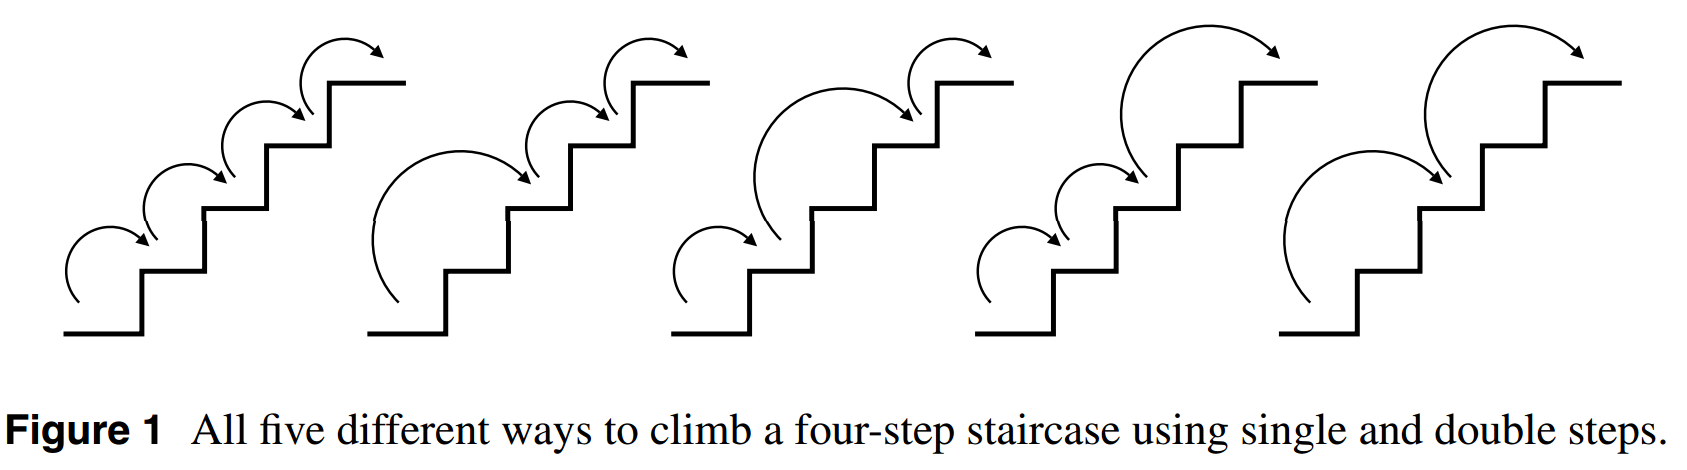
\includegraphics[scale=0.5]{/home/dspataro/git/algorithm_articles/sources/stairs_climbing/images/3stairs}
	\caption{All different ways to climb a 3 stairs staricase using steps of size $1$ or $2$.}
\end{figure}

\end{example}

\begin{example}
	\hfill \\
	Given $n = 4$ the answer is $5$ because there are five ways (See image \ref{fig:stair_example_5} to climb to the top of the stairs:
	\begin{enumerate}
		\item $1$ step + $1$ step + $1$ step + $1$ step
		\item $2$ steps + $1$ step + $1$ step
		\item $1$ step + $1$ step + $2$ steps 
		\item $1$ step + $2$ steps + $1$ step
		\item $2$ steps +  $2$ steps
	\end{enumerate}

\begin{figure}
	\label{fig:stair_example_5}
	\centering
	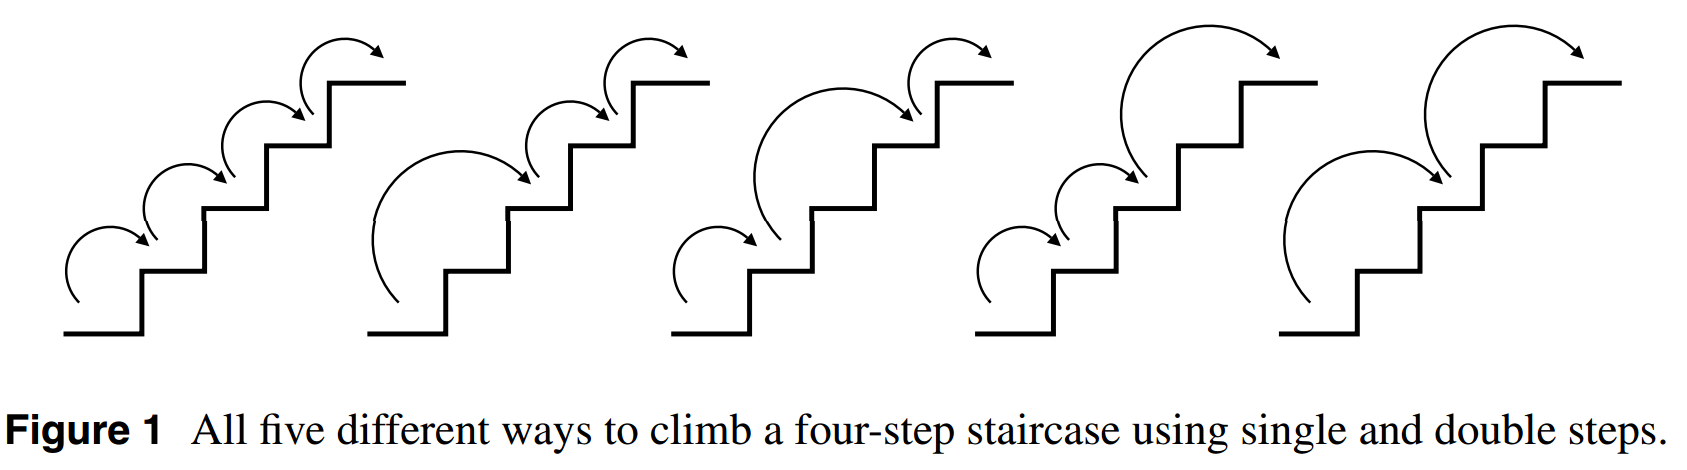
\includegraphics[scale=0.5]{/home/dspataro/git/algorithm_articles/sources/stairs_climbing/images/5stairs}
	\caption{All different ways to climb a four stairs staricase using steps of size $1$ or $2$.}
\end{figure}

\end{example}
	

\section{Clarification Questions}

\begin{QandA}
	\item Can the size of the stair be zero?
	\begin{answered}
		\textit{Yes, the staircase can be made of zero steps.}
	\end{answered}
	
	\item It is guaranteed the answer to fit a built-in integer?
	\begin{answered}
		\textit{Yes, do not worry about overflow.}
	\end{answered}

\end{QandA}

\section{Discussion}
\label{stairs_climbing:sec:discussion}

This is probably one problem that it is easier to tackle by first looking at a few examples so it is easier to see patterns. Table \ref{tab:stairs_climbing_ways_up_tp_7} shows  how many ways there are to climb a stair of lenght $n$ up to $n=7$.

\begin{table}
	\centering
	\begin{tabular}{|c|c|}
		\hline
		$n$ & \textbf{Ways} \\ \hline
		$0$ & $0$ \\ \hline
		$1$ & $1$ \\ \hline
		$2$ & $2$ \\ \hline
		$3$ & $3$ \\ \hline
		$4$ & $5$ \\ \hline
		$5$ & $8$ \\ \hline
		$6$ & $13$ \\ \hline
		$7$ & $21$ \\ \hline
	\end{tabular}
\label{tab:stairs_climbing_ways_up_tp_7}
\caption{All the ways to climb a stair of lenght $n \leq 7$ }
\end{table}

Looking at the table one thing should be immediately noticed i.e. the number of ways to climb the stair of size $n$ is equal to the $n^th$ element of the \textbf{Fibonacci} sequence (starting with two $1$).
Once tht is clear then the solution is straightforward as shown in Listing \ref{list:stairs_climbing_fibonacci}.

\lstinputlisting[language=c++, caption=Solution to the stairs climbining problem with steps of size $1$ and $2$ using Fibonacci.,label=list:stairs_climbing_fibonacci]{/home/dspataro/git/algorithm_articles/sources/stairs_climbing/stairs_climbing_solution1.cpp}

Now, let's have a look at why the seemingly unrelated fibonacci sequence plays a role in this problem. If the problem is looked at as an iterative process in which at each step a certain number of stairs are climbed. For instance if $n = 3$ and:
\begin{itemize}
	\item[-] $1$ step is hopped then the number of remaining steps is $3-1 = 2$. 
	\item[-] $2$ steps are hopped then the number of remaining steps is $3-2 = 1$.
\end{itemize}
When one step is hopped, the problem changes from climbing $n$ stairs to $n-1$ stairs. At this point the problem is seemingly unchanged except for the number of stairs left to climb and the same reasoning can be applied again:
\begin{itemize}
	\item[-] $1$ step is hopped then the number of remaining steps is $(n-1)-1 = n-2$. 
	\item[-] $2$ steps are hopped then the number of remaining steps is $(n-1)-2 = (n-3)$.
\end{itemize}
As can be seen, two decisions are possible i.e. climbing one or two stairs, exactly like in the fibinacci sequence, until either the $n$ step or a point past to it is reached.

\section{Common Variation
}
\subsection{Arbitrary step lengths}
\label{stairs_climbing:sec:arbitrary_steps}
But what happens when the step sizes allowed are not just $1$ or $2$ but an array of $k$ positive values $A=\{s_1 < s_2 < \ldots < s_k\}$. The problem statement for this harder variant of the problem is as follows:

\begin{exercise}
You are climbing a stair case and it takes $n$ steps to reach to the top.

Each time you can either climb $s_1$ or $s_2$ or $\ldots$ or $s_k$ steps where $0 < s_1 < s_2 < \ldots < s_k$. In how many distinct ways can you climb to the top?
\end{exercise}

Note how this problem is equivalent to the easier version described in Section \ref{sec:stairs_climbing_statement_easy} when the allowed step sizes are $s_i = 1$ and $s_2=2$.


	
\chapterimage{header}

\chapter{Permutations of an array}
\label{ch:permutations_array}
\section*{Introduction}
One of the topics that are commonly asked in interviews are finding certain permutations and combinations of data structures like arrays/vectors,etc. These topics really test the logical thinking abilities of a candidate and also help to gauge how good the candidate is in computer science fundamentals like recursion.

\section{Problem statement}
\begin{exercise}
Write a function (with signature: \lstinline[columns=fixed]{std::vector<std::vector<int> > array_permutations(std::vector<int> arr)} ) which takes in an array and returns all possible permutations of the input array.
\end{exercise}

\begin{example}
	   \hfill \\
	   Given $A=\{1,2,3\}$, the answer is 
	   $\{\{1,2,3\},\{1,3,2\},\{2,1,3\},\{2,3,1\},\{3,2,1\},\{3,1,2\}\}$
\end{example}

\section{Clarification Questions}
\begin{QandA}
	\item Are the inputs unique?
	\begin{answered}
		\textit{Yes, you can assume that the inputs are unique.}
	\end{answered}
	\item Can the array be empty?
	\begin{answered}
		\textit{No, It will contain atleast one element.}
	\end{answered}
\end{QandA}

\section{Discussion}

In order to compute all possible permutations, we need to first think about how the numbers can be arranged. Think that you have an array of size three, then for the first spot, you have three possible candidates. Once you place a candidate in the first spot, then for the second spot you are left with two possible candidates. Once the second spot is filled, you will have just one possible candidate for the last spot.So, the number of possible permutations for an array of size three would be $3 \times 2 \times \1 $. If you would remember from high school, the permutations of a given arrangement of size $n$ is given by $n!$. 

\subsection{Recursion}

One of the ways to compute the permutations of any arrangement is to approach this problem recursively. So, you could take the input array, swap the subsequent elements with the first element in the array. Then, you  could recursively do this until you reach the end of the array.

\lstinputlisting[language=c++, caption=Recursive solution to finding the permutations of an array ,label=list:permutations_array_recursive]{sources/permutations_array/permutations_array_recursive.cpp}


Another simple approach to this problem would be to just use \lstinline[columns=fixed]{std::next_permutation} from the standard template library. Though most interviewers would not accept this solution, mentioning this would give an impression that you are aware of the features of standard C++.

\lstinputlisting[language=c++, caption=Solution using C++ standard library]{sources/permutations_array/permutations_array_simple.cpp}

\section{Common Variations}
\subsection{Strings}
This same problem can be asked with strings as well. You can use the exact same approach for strings with no variations.
\subsection{Non unique Elements}
In this case, all that you would need to do is to keep only single occurence of non-unique elements in the array and generate permutations for the updated array.

\subsection{Permutations of exactly $k$ elements}
There could be instances where you could be asked to produce permutations of size $k$. In this case, you would need to  choose subarrays of size $k$ and then produce permutations for these sub-arrays.
	
    %%%%%%%%%%%%%%%%%%%%%%%%%%%%%%%%%%%%%%%%%%%%
	%               BIBLIOGRAPHY
	%%%%%%%%%%%%%%%%%%%%%%%%%%%%%%%%%%%%%%%%%%%%
	
	\chapter*{Bibliography}
	\addcontentsline{toc}{chapter}{\textcolor{ocre}{Bibliography}}
	\section*{Books}
	\addcontentsline{toc}{section}{Books}
	\printbibliography[heading=bibempty,type=book]
	\section*{Articles}
	\addcontentsline{toc}{section}{Articles}
	\printbibliography[heading=bibempty,type=article]
	
%%%%%%%%%%%%%%%%%%%%%%%%%%%%%%%%%%%%%%%%%%%%
%               INDEX
%%%%%%%%%%%%%%%%%%%%%%%%%%%%%%%%%%%%%%%%%%%%	
	\cleardoublepage
	\phantomsection
	\setlength{\columnsep}{0.75cm}
	\addcontentsline{toc}{chapter}{\textcolor{ocre}{Index}}
	\printindex


	%\backmatter

\end{document}